
\chapter{Estudio teórico}
\label{cha:estudio-teórico}

\begin{FraseCelebre}
  \begin{Frase}
    Si buscas resultados distintos no hagas siempre lo mismo.
  \end{Frase}
  \begin{Fuente}
    Albert Einstein
  \end{Fuente}
\end{FraseCelebre}

\section{Introducción}
\label{sec:intro-sota}

En este capítulo se ha realizado un estudio del marco teórico que engloba este trabajo donde se revisará los últimos estudios relacionados con los sistemas de detección de objetos abandonados. 

En primer lugar, se ha realizado un repaso de las diferentes técnicas que se han utilizado hasta día de hoy en la detección de objetos abandonados en imágenes. La segmentación de objetos en movimiento situados en primer plano, la detección de objetos estacionarios, el reconocimiento de comportamientos o la detección de personas y objetos mediante el uso de \gls{cnn} son los métodos de detección más relevantes en los últimos años.

En segundo lugar, se hará una breve introducción a las \gls{cnn}, un tipo de red neuronal artificial de \textit{Deep Learning}, que utiliza imágenes en la entrada de la red para encontrar patrones en las imágenes con el objetivo de reconocer formas dentro de los objetos. También resulta interesante su uso en la clasificación de datos de audio o señales. En los últimos años se están utilizando para el reconocimiento facial o vehículos autónomos.

Por último, y más enfocado a los contenidos de este trabajo, se extenderá la sección \ref{subsec:tecnicas-deteccion-personas-objetos} realizando un breve recorrido por los principales algoritmos de detección y seguimiento de personas y objetos basados en \gls{cnn}.

\section{Estado del Arte}
\label{sec:estado-del-arte}

En esta sección se va a enumerar las distintas técnicas que han sido utilizadas en la identificación de objetos abandonados citando los trabajos más relevantes de otros investigadores.

\subsection{Segmentación de objetos en primer plano}
\label{subsec:tecnicas-segmentacion-obj-primer-plano}

El análisis de vídeo se trata de uno de los campos de investigación más amplios en la actualidad. Muchas de las aplicaciones han necesitado tener un primer paso en la detección de movimiento de objetos en un escenario como en \cite{cheung2005robust}, donde se ha realizó una sustracción del fondo para la videovigilancia de tráfico urbano o en espacios de aprendizaje multimedia \cite{4381122}. Una etapa básica en estos sistemas se trata de la separación de los objetos que se encuentran en un primer plano con el fondo.

Típicamente, la forma de modelar el fondo es obtener una imagen que se encuentre en el fondo sin ningún objeto en movimiento \cite{BOUWMANS201431}. En ocasiones el modelo de representación debe de ser robusto, ya que nos podemos encontrar con fondos de escenarios que sufran cambios debidos a alteraciones en la iluminación u objetos que han sido introducidos y/o retirados.

Por tanto, los dos principales problemas con los que nos encontramos en la sustracción del fondo son la detección de cambios y la detección de movimientos. Cuando hablamos de detección de cambios hablamos de los cambios producidos entre dos imágenes. Cuando se realiza una sustracción del fondo podemos encontrarnos con dos casos, que una imagen corresponda al fondo y la otra imagen corresponda a la imagen actual, o bien que los cambios se han producido por el movimiento de las personas u objetos.

En la figura \ref{fig:background-subtraction-process} se muestra las etapas de la sustracción del fondo donde inicialmente se emplean N fotogramas para obtener la imagen del fondo sin que haya ningún objeto en movimiento. La siguiente etapa corresponde a la detección de objetos en movimiento en el primer plano donde se clasifica los píxeles que se encuentran en el primer plano comparando el fondo con la fotograma actual. Hay una etapa de mantenimiento para actualizar la imagen del fondo en todo momento. Estas dos últimas etapas nombradas se realizan en bucle a lo largo del tiempo.

\begin{figure}[ht]
\centering
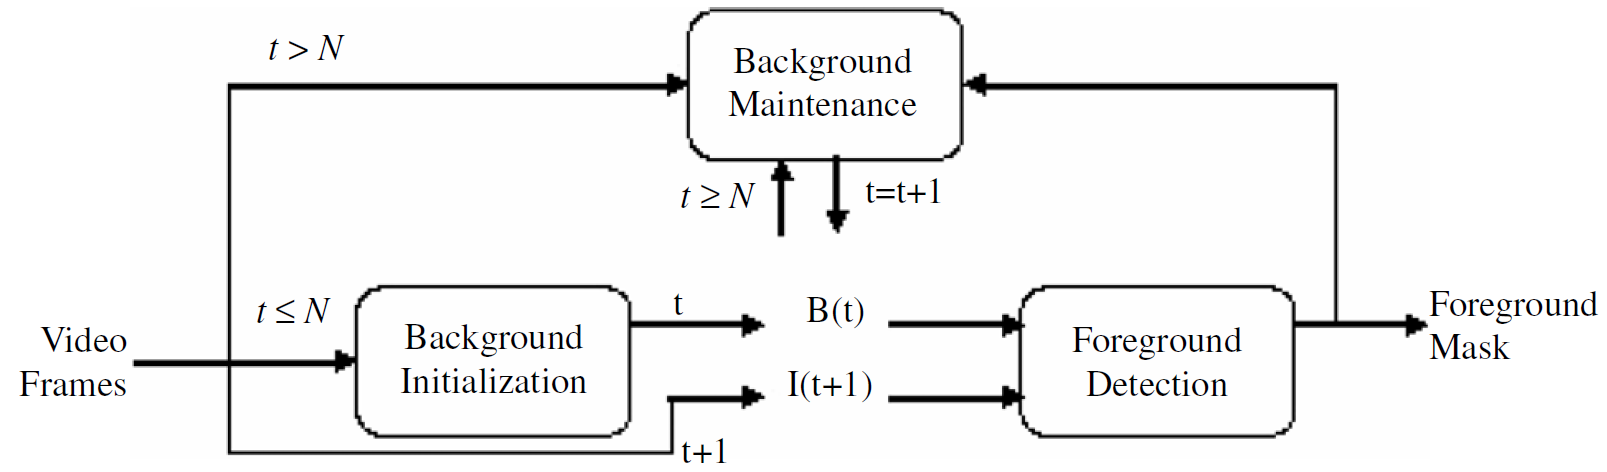
\includegraphics[width=0.85\textwidth]{img/chapters/estado-del-arte/background-subtraction-process.png}
\caption{\label{fig:background-subtraction-process}Proceso de la sustracción del fondo \cite{BOUWMANS201431}}
\end{figure}

A continuación, se exponen con más detalle cada una de las etapas que compone la sustracción del fondo:

\subsubsection*{Inicialización del fondo}
\label{subsubsec:inicializacion-del-fondo}

Consiste en el modelado del fondo donde se describe el tipo de modelo que se está utilizando para representar. Principalmente se determina la capacidad del modelo para tratar con fondos estáticos (unimodal) o fondos dinámicos (multimodal).

En esta etapa se inicializa el modelo donde generalmente se utiliza el primer fotograma sobre un conjunto de fotogramas de entrenamiento, los cuales contienen o no objetos en primer plano. El principal desafío es obtener un primer modelo de fondo cuando más de la mitad de los fotogramas entrenamiento contiene objetos en primer plano.


\subsubsection*{Mantenimiento de fondo}
\label{subsubsec:mantenimiento-fondo}

El mantenimiento del fondo se encarga de adaptar el modelo a los cambios que puedan ser ocasionados a lo largo del tiempo. En esta etapa de aprendizaje se debe de realizar en línea por lo que el algoritmo debe de ser incremental. Los puntos claves en este proceso son los siguientes:

\begin{itemize}
    \item \textbf{Esquemas de mantenimiento}. En trabajos previos como en \cite{4712338} se presentan tres esquemas de mantenimientos: ciegos, selectivos y adaptativos difusos. El mantenimiento ciego del fondo actualiza todos los píxeles con las mismas reglas que se emplean en un filtro IIR:
    
    \begin{equation}
    \label{eq:IIR-filter}
    \text{B}_{t+1}(x,y) = (1 - \alpha)\text{B}_{t}(x,y) + \alpha\text{I}_{t}(x,y)
    \end{equation}
    
    donde:
    
    \begin{itemize}
        \item $\alpha$ es el ratio de aprendizaje y tiene un valor comprendido entre [0,1].
        \item $\text{B}_{t}$ y $\text{I}_{t}$ son el fondo y la imagen actual respectivamente en el tiempo t.
    \end{itemize}
    
    La principal desventaja de este esquema es que el valor de los píxeles clasificados como primer plano son utilizados en el cálculo del nuevo fondo y por tanto, afecta a la imagen de fondo. Para lidiar con este problema algunos investigadores utilizan un esquema de mantenimiento selectivo que se basa en actualizar la nueva imagen de fondo con diferentes ratios de aprendizaje en función de la clasificación previa del píxel en primer plano o fondo:
    
    \vspace{0.5cm}

    $\text{B}_{t+1}(x,y) = (1 - \alpha)\text{B}_{t}(x,y) + \alpha\text{I}_{t}(x,y)$
    
    \vspace{0.5cm}
    
    si $(x,y)$ es el fondo
    
    \vspace{0.5cm}

    $\text{B}_{t+1}(x,y) = (1 - \beta)\text{B}_{t}(x,y) + \beta\text{I}_{t}(x,y)$
    
    \vspace{0.5cm}
    
    si $(x,y)$ es el primer plano
    
    \vspace{0.5cm}
    
    La idea es adaptar el píxel clasificado como fondo de manera rápida y un píxel clasificado como primer plano muy despacio. Por está razón $\beta \ll \alpha$ y generalmente $\beta = 0$. Por tanto, la ecuación \ref{eq:IIR-filter} se convierte en:
    
    \begin{equation}
    \label{eq:IIR-filter2}
    \text{B}_{t+1}(x,y) = \text{B}_{t}(x,y)
    \end{equation}
    
    El problema es que una clasificación errónea puede resultar un error permanente en el modelo del fondo. Este problema se puede solucionar mediante un esquema adaptativo difuso que toma en cuenta la incertidumbre de la clasificación. Esto puede lograrse graduando la regla de actualización utilizando el resultado de la detección del primer plano.
    
    \item \textbf{Ratio de aprendizaje}. Determina la velocidad de adaptación en los cambios de escena. Este ratio puede ser fijo, ajustado dinámicamente o difuso.
    \item \textbf{Mecanismos de mantenimiento}. El ratio de aprendizaje determina la velocidad de adaptación a los cambios de iluminación pero también el tiempo que necesita un cambio en el fondo hasta que se incorpora en el modelo, así como el tiempo donde un objeto que se encuentra en el primer plano estático puede sobrevivir antes de ser incluido en el modelo. El ratio de aprendizaje por tanto se encarga de diferentes desafíos diferenciados. Para desacoplar el mecanismo de adaptación y el de incorporación, \cite{1415580} se utilizó un conjunto de contadores que representan el número de veces que un píxel se clasifica como píxel de primer plano. Cuando este número es mayor que cierto umbral, el píxel se considera que se encuentra en el fondo. Esto da un límite de tiempo de cuanto tiempo un píxel se encuentra como píxel del primer plano estático.
    \item \textbf{Frecuencia de actualización}. El objetivo es actualizar el fondo solo cuando sea necesario. El mantenimiento se puede realizar en cada fotograma, sin embargo si no se producen cambios no es necesaria la actualización de los píxeles en cada fotograma.
\end{itemize}

\subsubsection*{Detección del primer plano}
\label{subsubsec:detección-primer-plano}

Esta etapa se trata de una tarea de clasificación que se encarga de etiquetar píxeles como fondo o como píxeles de primer plano.

\subsubsection*{Aplicaciones donde se utiliza la sustracción del fondo}
\label{subsubsec:aplicaciones-background-subtraction}

La segmentación de objetos en movimiento sobre el primer plano se utiliza en multitud de aplicaciones donde se emplea visión por computadora como pueden ser:

\begin{itemize}
    \item \textbf{Videovigilancia inteligente}. Se trata de una de las aplicaciones donde más se utiliza esta metodología. El objetivo es detectar objetos en movimiento u objetos abandonados para garantizar la seguridad aérea, para calcular estadísticas de tráfico como se puede ver en la figura \ref{fig:background-subtraction-example} o para vigilancia marítima. Los objetos de interés suelen ser variados como vehículos, aviones, barcos, personas o equipajes.
    \item \textbf{Codificación de vídeo basada en el contenido}. Para generar un vídeo, debe de estar segmentado en objetos de vídeo y seguidos a medida que transcurren los fotogramas del vídeo. El fondo y los objetos presentes en el vídeo son codificados por separado. En definitiva, la codificación en vídeo necesita métodos efectivos para la detección de objetos en entornos estáticos y dinámicos.
    \item \textbf{Captura de movimiento óptico}. El objetivo es obtener una captura completa y precisa de las personas mediante el uso de cámaras. La silueta se extrae generalmente en cada vista de la sustracción del fondo.
\end{itemize}

\begin{figure}[ht]
\centering
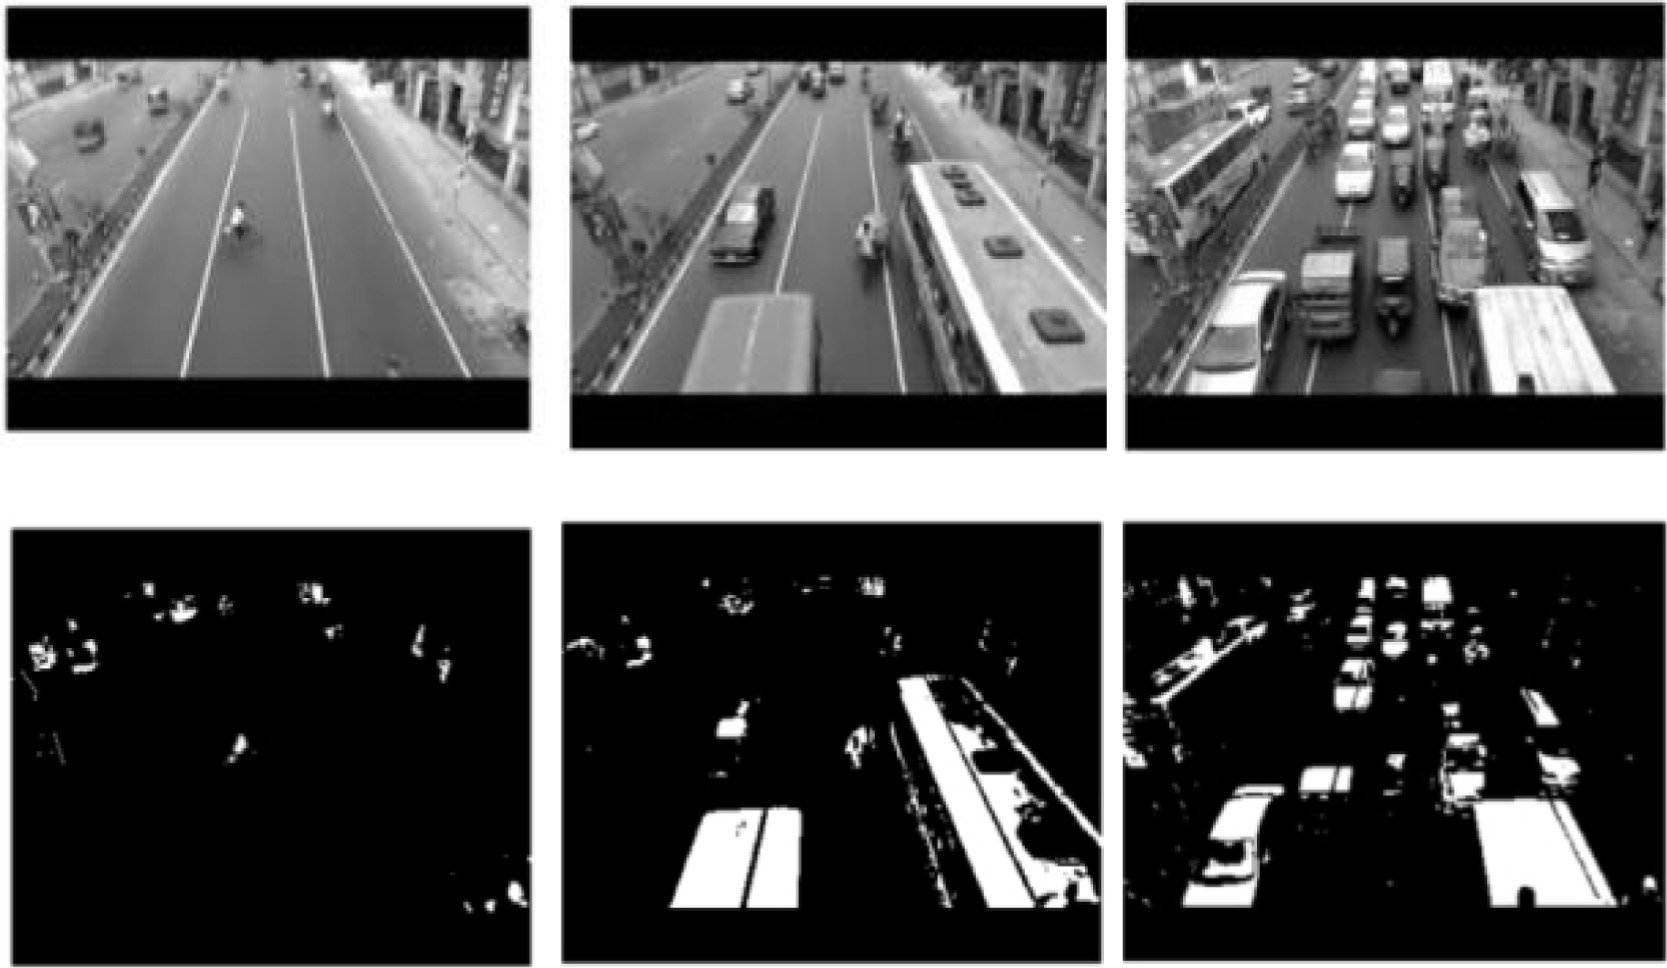
\includegraphics[width=0.55\textwidth]{img/chapters/estado-del-arte/background-subtraction-example.jpg}
\caption{\label{fig:background-subtraction-example}Ejemplo de sustracción del fondo en aplicaciones de tráfico \cite{BOUWMANS201431}}
\end{figure}

\subsection{Detección de objetos estacionarios}
\label{subsec:tecnicas-deteccion-obj-estacionarios}

La detección de objetos estacionarios está recibiendo una atención especial ya que se trata de una fase de análisis crítico en aplicaciones como la detección de objetos abandonados o vehículos estacionados en áreas públicas. El reconocimiento de objetos estacionarios en escenarios de grandes aglomeraciones de personas supone una tarea desafiante.

Se producen problemas ocasionados por las oclusiones o variación de colores y formas conforme las personas se mueven. Otros problemas que surgen son la iluminación, la velocidad de los objetos y la densidad de los objetos se deben de tener en cuenta. En la detección de objetos en primer plano, los métodos basados en la sustracción de fondo se han vuelto muy populares debido a que se suelen emplear cámaras fijas y los cambios de iluminación son muy graduales \cite{1217925}. En trabajos previos como en \cite{5279450} se propone enfoque en el análisis de imágenes estáticas.

En la figura \ref{fig:metodos-sustraccion-objeto-estacionario} se muestra clasificación de sustracción del fondo en base al método utilizado.

\begin{figure}[ht]
\centering
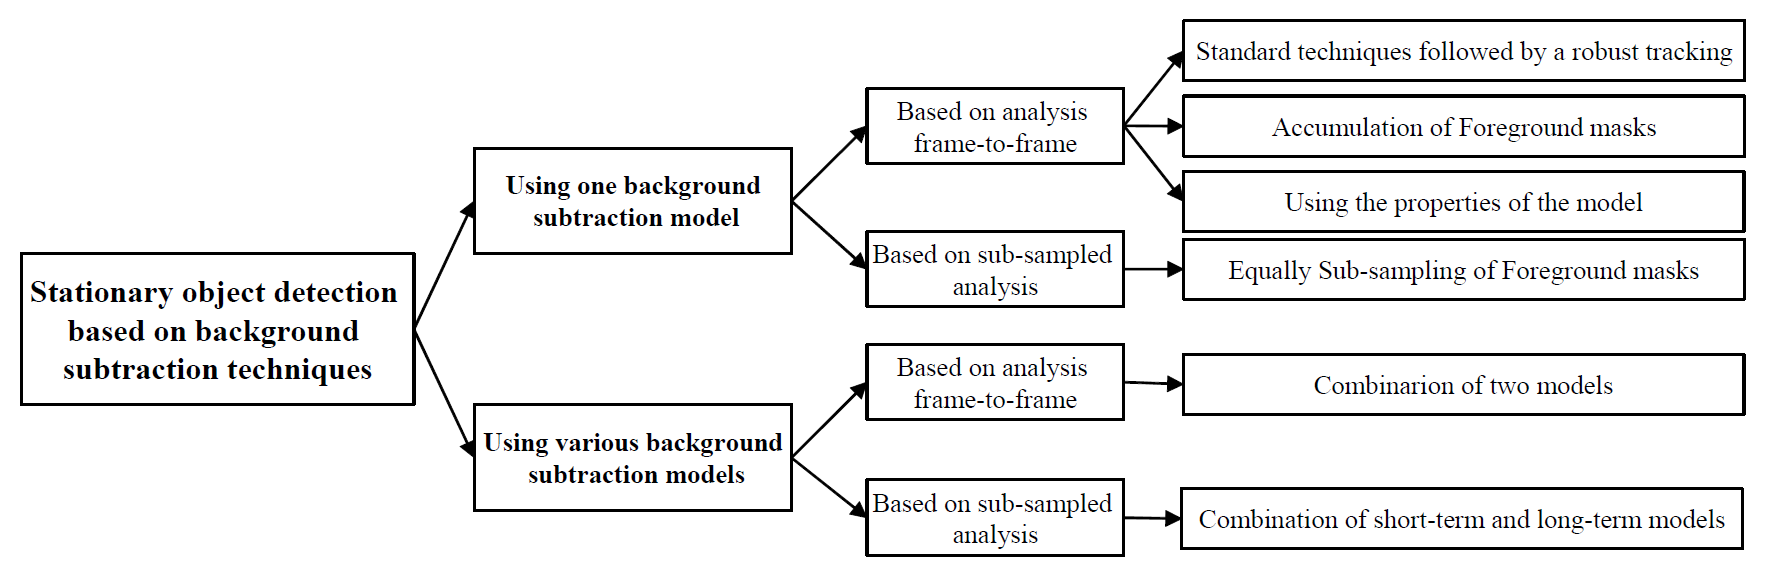
\includegraphics[width=0.95\textwidth]{img/chapters/estado-del-arte/metodos-sustraccion-fondo-deteccion-fondo-estacionario.png}
\caption{\label{fig:metodos-sustraccion-objeto-estacionario}Clasificación de sustracción del fondo basados en métodos de detección de objetos estacionarios \cite{5279450}}
\end{figure}

Dependiendo del uso de los mapas en primer plano calculados en el análisis de sustracción de fondo, los enfoques basados en un modelo se pueden clasificar en:

\begin{itemize}
    \item \textbf{Basado en análisis fotograma a fotograma}. Se emplean técnicas de sustracción del fondo seguidas de otro tipo análisis. En función de este tipo de análisis se puede clasificar en: basados en el uso de técnicas estándar de fondo seguido de otra etapa de análisis, basados en la acumulación de máscaras en primer plano calculadas fotograma a fotograma, o basado en las propiedades del modelo de sustracción de fondo utilizado.
    \item \textbf{Basado en análisis de submuestreo}. Estas propuestas tratan de detectar objetos estacionarios analizando las secuencias de vídeos a diferentes velocidades de fotogramas. 
\end{itemize}

Los enfoques que combinan uno o más modelos de sustracción de fondo han sido menos estudiados. No obstante, una clasificación basada en el procesamiento de la velocidad de los fotogramas se puede realizar de la siguiente manera:

\begin{itemize}
    \item \textbf{Basado en análisis fotograma a fotograma}. En esta categoría tenemos métodos que combinan diferentes propiedades usando dos o varias técnicas de sustracción de fondo.
    \item \textbf{Basado en un análisis de submuestreo}. Estos enfoques detectan objetos estacionarios analizando las secuencias de vídeo con varios métodos de sustracción de fondo a diferentes velocidades de fotogramas.
\end{itemize}

\subsection{Detección de personas y objetos}
\label{subsec:tecnicas-deteccion-personas-objetos}

Existe una gran cantidad de estudios de detección de personas en la literatura, algunos de ellos cubren parcialmente solo el Estado del Arte o están claramente enfocados en alguna aplicación de videovigilancia en particular. En \cite{4657363} se presenta un estudio de detección de personas y también la integración de los detectores en sistemas completos a bordo. Descompone los enfoques de detección de personas en tres tareas de procesamiento: generación de hipótesis de objeto inicial o selección de la \gls{roi}, verificación (clasificación) e integración temporal (seguimiento). \cite{simonnet2012} presenta una descripción general de los algoritmos de detección de personas centrados solo en enfoques de búsqueda exhaustivos, mientras que en \cite{5975165} presentan una descripción general centrada únicamente en enfoques de ventana deslizante.

Se pueden clasificar los algoritmos de detección de personas en: las técnicas utilizadas, el tipo de modelos utilizados, el uso de información 2D o 3D, la modalidad del sensor, la multiplicidad del sensor, la ubicación del sensor o la movilidad del sensor. Los algoritmos de detección de personas se clasifican según el enfoque utilizado para generar o extraer los objetos iniciales y en base al modelo de persona.

\subsubsection*{Hipótesis de objeto inicial}
\label{subsubsec:hipotesis-inicial-deteccion-personas-objetos}

Hay dos enfoques principales de detección de objetos convencionales (ver figura \ref{fig:people-detection-classification}): los que se basan en algún tipo de segmentación de la escena en primer plano (objetos) y el fondo \cite{868681} y los que se basan en un enfoque de búsqueda exhaustiva \cite{4408936}. También hay algunos enfoques que intentan combinar ambas técnicas juntas \cite{4220664}. El resultado de esta etapa es la ubicación y dimensión (cuadro delimitador) de los diferentes objetos de la escena candidatas a ser una persona.

\begin{figure}[ht]
\centering
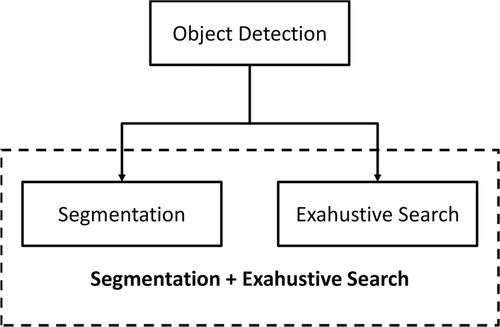
\includegraphics[width=0.4\textwidth]{img/chapters/estado-del-arte/people-detection-classification.png}
\caption{\label{fig:people-detection-classification}Clasificación de detección de personas enfocado a la detección de objetos \cite{https://doi.org/10.1049/iet-cvi.2014.0148}}
\end{figure}

\paragraph*{Segmentación}\mbox{} \\
\label{parag:deteccion-objetos-personas-segmentacion}

El uso de la segmentación genera directamente los objetos candidatos a ser persona y fácilmente se rechaza las áreas irrelevantes de la imagen, es decir, sin objetos de interés. Por este motivo, la tarea de clasificación posterior se simplifica claramente y, por tanto, el modelo de persona suele ser más sencillo y de menor coste computacional. Sin embargo, como existe una fuerte dependencia de la segmentación, todos los problemas de segmentación se heredan (segmentaciones por debajo y por encima). Estos problemas pueden afectar el rendimiento de la detección global, principalmente limitando la tasa máxima de detección (objetos no detectados) pero también aumentando el número de detecciones falsas (detecciones de objetos parciales u objetos superpuestos). Además, estos problemas se magnifican en escenarios complejos donde es bastante difícil obtener una segmentación confiable.

\paragraph*{Búsqueda exhaustiva}\mbox{} \\
\label{parag:deteccion-objetos-personas-busqueda-exhaustiva}

La otra técnica para obtener la hipótesis de ubicación inicial del objeto es la búsqueda exhaustiva. Por lo general, consiste en escanear la imagen completa buscando similitudes con el modelo de persona elegido en múltiples escalas y ubicaciones. A través de este mecanismo se obtiene un mapa de confianza de detección denso (escala y ubicación). Para llegar a detecciones individuales, estos enfoques deben buscar máximos locales en el volumen de densidad y luego aplicar alguna forma de supresión no máxima.

Hay muchas propuestas de detección de personas en el Estado del Arte que utilizan esta técnica, de hecho, esta técnica es actualmente la más utilizada. Dentro de esta técnica, se pueden utilizar dos enfoques diferentes como se expone en \cite{5674059}. Existen algunas propuestas que obtienen este volumen de densidad implícitamente muestreando en una cuadrícula 3D discreta (ubicación y escala) evaluando diferentes ventanas de detección con un clasificador. Este es el caso del uso de detectores basados en ventanas deslizantes como en \cite{4409057}.

\subsubsection*{Modelos de personas}
\label{subsubsec:modelos-personas-deteccion-personas-objetos}

El proceso de verificación o clasificación aplica un modelo de persona previamente definido o entrenado a los objetos candidatos a ser persona a partir de una imagen o secuencia y toma una decisión final en función de su similitud. Por lo tanto, la definición de un modelo de persona adecuado es una tarea crítica para el proceso de verificación o clasificación. Hay dos fuentes principales de información discriminativa para caracterizar el modelo de personas: apariencia y movimiento (ver figura \ref{fig:people-detection-people-model}). El modelo debería poder discriminar entre personas y cualquier otro objeto en la escena.

\begin{figure}[ht]
\centering
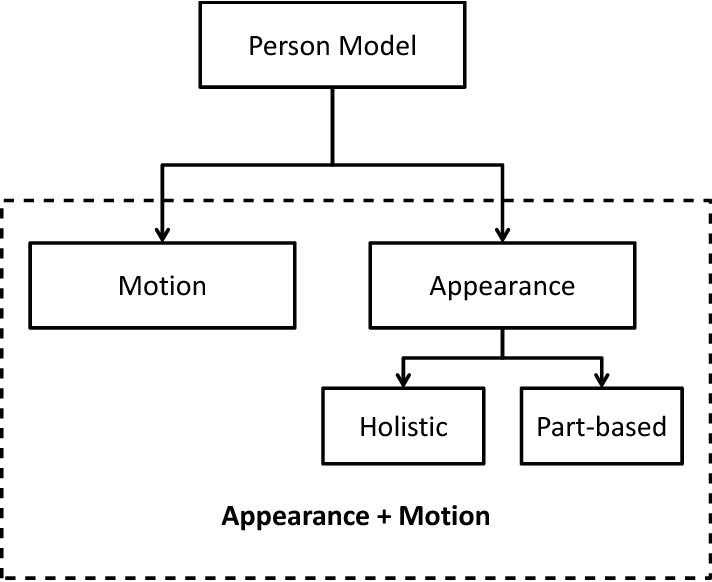
\includegraphics[width=0.4\textwidth]{img/chapters/estado-del-arte/people-detection-people-model.png}
\caption{\label{fig:people-detection-people-model}Clasificación de detección de personas según modelo de persona \cite{https://doi.org/10.1049/iet-cvi.2014.0148}}
\end{figure}

\paragraph*{Basado en el movimiento}\mbox{} \\
\label{parag:basado-movimiento-people-model}

La apariencia humana varía debido a factores ambientales como las condiciones de luz, vestimenta o contrastes. Además de la enorme variabilidad intrínseca de las personas como diferentes alturas, anchos o poses. Por estas razones, existen algunos enfoques que intentan evitarlos utilizando sólo información de movimiento. Dentro de esta clasificación, \cite{868681} proponen un sistema de clasificación de objetos basado en análisis de movimiento periódico. El algoritmo segmenta el movimiento, rastrea los objetos en primer plano, alinea cada objeto a lo largo del tiempo y finalmente calcula la auto-similitud entre los objetos y cómo evoluciona en el tiempo. \cite{1334092} propone un sistema de detección de personas basado en la detección de patrones de movimiento de personas. Para cada objeto presente en dos imágenes consecutivas, se realiza la normalización de tamaño y se calcula su patrón de flujo que consiste en flujos ópticos horizontales y verticales.

\paragraph*{Basado en apariencia}\mbox{} \\
\label{parag:basado-apariencia-people-model}

Hay muchos enfoques que utilizan información de apariencia para definir el modelo de persona. Esto se debe a que la apariencia discrimina más que el movimiento. Los modelos de apariencia se clasifican según modelos humanos simplificados o modelos complejos. Existen modelos de persona simples que definen a la persona como una región o forma, es decir, modelos holísticos \cite{1334092} y modelos más complejos que definen a la persona como una combinación de múltiples regiones o formas, es decir, modelos basados en piezas \cite{5255236}.

\subsection{Reconocimiento del comportamiento}
\label{subsec:tecnicas-reconocimiento-comportamiento}

La detección de un comportamiento anormal en la videovigilancia es esencial para garantizar la seguridad tanto en lugares interiores como exteriores, como estaciones de trenes o aeropuertos. La detección de conductas anormales es un problema particular del reconocimiento de la acción humana. Con el creciente número de cámaras de vigilancia, la tarea de supervisar múltiples monitores por parte del personal de seguridad se vuelve muy difícil debido a la falta de atención y a la fatiga humana. Además, los eventos anormales son relativamente raros y no ocurren con frecuencia. Esto hace que la tarea de supervisión sea más compleja. Por tanto, existe una demanda creciente de un sistema de videovigilancia inteligente que detecte de manera automática los comportamientos anormales y avise mediante una alarma.

En esta sección se va a revisar los métodos existentes \cite{BENMABROUK2018480} que se utilizan en aplicaciones de videovigilancia destacando los avances actuales en el campo de la detección de comportamientos anormales. El objetivo de un sistema de videovigilancia inteligente es detectar de manera eficiente un evento interesante a partir de una gran cantidad de vídeos para prevenir situaciones peligrosas. Esta tarea requiere dos niveles de procesamiento de vídeo tal y como se muestra en la figura \ref{fig:video-surveillance-system}.

\begin{figure}[ht]
\centering
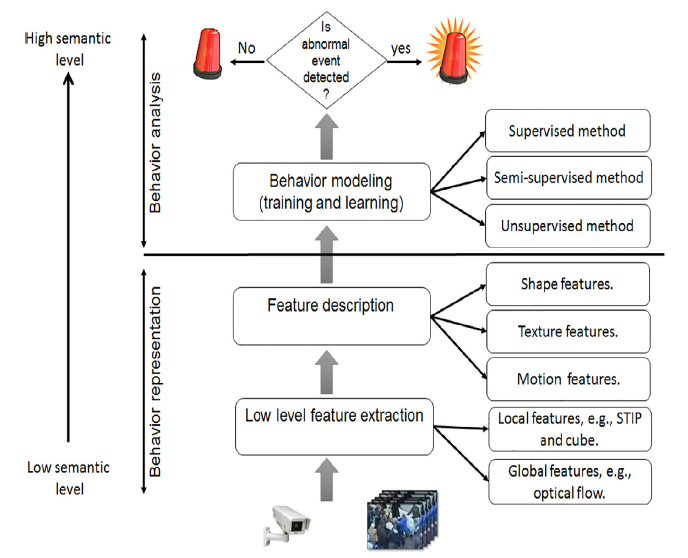
\includegraphics[width=0.6\textwidth]{img/chapters/estado-del-arte/video-surveillance-system.png}
\caption{\label{fig:video-surveillance-system}Sistema de videovigilancia inteligente \cite{BENMABROUK2018480}}
\end{figure}

El primero consta de dos pasos. Primero, se extraen características de bajo nivel, con el objetivo de detectar la \gls{roi} en la escena. Luego, se generan primitivas basadas en características de bajo nivel para describir la \gls{roi}. El segundo nivel proporciona información semántica sobre la acción humana y determina si el comportamiento es normal o no.

La detección de comportamientos anormales en la videovigilancia es una tarea desafiante en la visión por computadora y últimamente ha experimentado importantes avances. Las etapas de procesamiento de bajo nivel permiten detectar y describir el objeto en movimiento en la escena. Sin embargo, esos pasos no permiten comprender el tipo de acción que realiza el objeto en movimiento ni determinar si su comportamiento es normal o no. Dado que existen múltiples trabajos propuestos que se relacionan con el reconocimiento de conductas anormales en la videovigilancia, en esta sección se va a hacer una revisión de:

\begin{itemize}
    \item Modelado de marcos y métodos de clasificación.
    \item Densidad de escenas e interacción de objetos en movimiento.
\end{itemize}

\subsubsection*{Modelado de marcos y métodos de clasificación}
\label{subsubsec:modelado-frameworks-métodos-clasificación}

El reconocimiento de un comportamiento anormal depende del marco de referencia propuesto y del método utilizado para clasificar los comportamientos. Dado el tipo de muestras requeridas para el proceso de aprendizaje (normal o anormal), los métodos de clasificación se pueden categorizar en métodos supervisados, semi-supervisados y no supervisados.

Los métodos supervisados tienen como objetivo modelar comportamientos normales y anormales a través de datos etiquetados. Por lo general, están diseñados para detectar comportamientos anormales específicos predefinidos en la fase de entrenamiento, como la detección de enfrentamiento entre personas, la detección de merodeos y detección de caídas. En la literatura se proponen varios métodos supervisados con el objetivo de detectar un evento interesante en un vídeo. Uno de los más populares es el enfoque \gls{bow} \cite{ACAMPORA2015130}. Consiste en representar cada vídeo o fotograma mediante un histograma de palabras. Primero, se construye un diccionario de palabras. Luego, el histograma se calcula contando la frecuencia de cada palabra dentro del diccionario en el vídeo. El enfoque \gls{bow} se usa generalmente con el clasificador de \gls{svm}, que es una herramienta eficiente para la detección de comportamiento agresivo y el reconocimiento de anomalías de multitudes.

Los métodos semi-supervisados solo necesitan datos de vídeo normales para el entrenamiento y se pueden dividir en categorías basadas en reglas y basadas en modelos. La primera categoría tiene como objetivo desarrollar una regla utilizando patrones normales. Cualquier muestra que no se ajuste a esta regla se considera un valor atípico (anomalía). En \cite{6751449} se propuso un método basado en reglas que utiliza codificación escasa para detectar comportamientos anormales. Aunque se logró un buen resultado en un tiempo de ejecución corto (150 \gls{fps}), su resultado se ve muy afectado por el valor de umbral. Otros trabajos se basan en la construcción de algunas reglas para clasificar el comportamiento en normal y anormal. En \cite{6931308} se propone un sistema de detección de caídas basado en reglas extraídas utilizando características de forma.

Los métodos no supervisados tienen como objetivo aprender comportamientos normales y anormales utilizando propiedades estadísticas extraídas de datos no etiquetados. En \cite{alvar2014} propusieron un método de comportamiento anormal utilizando un marco de aprendizaje no supervisado basado en Dominant Set. En \cite{Ren2013UnsupervisedKL} presentaron un marco de kernel no supervisado para la detección de anomalías basado en el espacio de características y la \gls{svdd}.


\subsubsection*{Densidad de escenas e interacción de objetos en movimiento}
\label{subsubsec:densidad-escenas-interacción-objetos-movimiento}

La densidad de la escena corresponde al número de personas presentes en ella. La elección de las técnicas a utilizar para caracterizar el comportamiento está directamente influenciada por la densidad de la escena. Por lo tanto, el objeto en movimiento en la escena puede ser un pequeño número de personas o un grupo de personas. Se distinguen dos tipos de escenas. El primer tipo, llamado escena con poca gente, se caracteriza por la presencia de una o unas pocas personas al mismo tiempo dentro del campo de visión de la cámara. El segundo tipo se llama escena llena de gente, ya que contiene muchas personas.

\paragraph*{Escena con poca gente}\mbox{} \\
\label{parag:escena-poca-gente}

En este tipo de escenas, es interesante detectar un comportamiento anormal realizado por una o varias personas presentes dentro del campo de la cámara. Cuando solo hay una persona en la escena, generalmente se consideran tres comportamientos anormales principales que son detección de caída, merodeo y estar en un lugar equivocado (ver figura \ref{fig:abnormal-behaviors-single-person}).

\begin{figure}[ht]
\centering
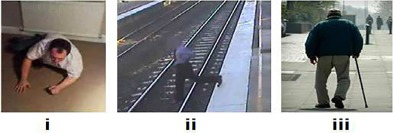
\includegraphics[width=0.45\textwidth]{img/chapters/estado-del-arte/Abnormal-behaviors-single-person.jpg}
\caption{\label{fig:abnormal-behaviors-single-person}Comportamientos anormales realizados por una sola persona \cite{BENMABROUK2018480}}
\end{figure}

La detección de caídas humanas es una tarea interesante y varios trabajos propusieron sistemas que se utilizan para garantizar la seguridad y protección, especialmente para las personas mayores y para las personas que viven solas. En \cite{6804646}, se propone un método de rastreo de partes del cuerpo humano para detectar caídas de personas mayores. Utilizaron solo una cámara de profundidad que hace que la aproximación funcione incluso en la oscuridad. En \cite{HUANG2014125}, se propone un algoritmo que es capaz de reconocer el comportamiento anormal de las personas mayores solitarias a partir de la información obtenida de un espacio inteligente. En \cite{6916753} propusieron un nuevo sistema para monitorear a las personas solas (personas mayores, pacientes que viven solos, etc.) mediante la explotación de la información de imagen y audio en vídeo para detectar eventos anormales.

Otro tema interesante en la escena con poca gente merodeando. Se entiende merodear como el acto de estar durante un largo período en un espacio público en particular sin ningún objetivo, como que una persona tenga una maleta en un aeropuerto y se quede mucho tiempo sin ningún propósito. Este acto es anormal y varios trabajos propusieron diferentes técnicas para detectar la ocurrencia de este evento. En \cite{10.1007/978-3-319-18914-7_54} se propuso un sistema de detección de merodeo de dos etapas basado en micropatrones secuenciales. Esos micropatrones son acciones repetidas realizadas por un individuo que caracteriza el comportamiento de merodeo y se obtienen con el algoritmo de patrones secuenciales generalizados. En \cite{6959931} proponen un método para detectar merodeo en videovigilancia utilizando el historial de direcciones de la trayectoria del objeto en movimiento y el método de \gls{ipm}.

\paragraph*{Escena llena de gente}\mbox{} \\
\label{parag:escena-llena-gente}

En este tipo de escena, no es posible rastrear y analizar el comportamiento de cada persona de forma individual. Esto se debe a la oclusión y al pequeño número de píxeles que representan a cada persona en el fotograma. Por ello, es mejor modelar la interacción entre personas para detectar un comportamiento anormal de la multitud. Varios trabajos previos propusieron métodos de detección de comportamientos anormales en escenarios llenos de personas basados en la interacción entre personas. La figura \ref{fig:abnormal-behaviors-crowded-scene} muestra algunos comportamientos anormales de la multitud.

\begin{figure}[ht]
\centering
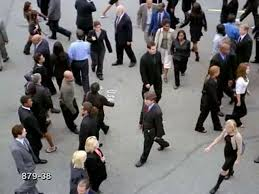
\includegraphics[width=0.4\textwidth]{img/chapters/estado-del-arte/abnormal-behaviors-crowded-scene.jpg}
\caption{\label{fig:abnormal-behaviors-crowded-scene}Comportamientos anómalos en multitudes}
\end{figure}

La interacción grupal incluye comportamientos realizados por varias personas, como el causado por el pánico grupal y la violencia en el estadio de fútbol. Muchos trabajos se enfocaron en detectar eventos inusuales que ocurren en escenas concurridas. En \cite{5206641} se propuso un método para detectar el comportamiento anormal de la multitud utilizando un modelo de fuerza social que estima la fuerza de interacción entre individuos. Primero, calcularon el modelo de fuerza social y luego usaron el enfoque \gls{bow} para clasificar los eventos como normales y anormales. En \cite{6202466} propusieron un método para la detección de anomalías utilizando múltiples modelos de comportamiento social que se determinan en función del flujo óptico y la advección de partículas. En \cite{CHO201464} utilizaron agentes estáticos y dinámicos para caracterizar la interacción grupal. Los agentes estáticos tienen como objetivo observar los comportamientos individuales calculando la variación del flujo óptico. Los agentes dinámicos calculan la interacción grupal utilizando el modelo de fuerza social. En \cite{7019309} se basan en la detección y el análisis de movimiento para describir la anomalía. En \cite{6910023} proponen un método de detección de grupos sociales en una escena abarrotada basado en dos características que son la dirección de la mirada y la atención visual. Esas dos características se utilizan para especificar la intención de la persona en el vídeo.

En \cite{6239348} detectaron la violencia de masas en tiempo real basándose en un nuevo detector Violent Flows. En \cite{CHAKER2017266} se introdujeron un marco no supervisado basado en el modelo de red social para capturar la interacción de la multitud y la dinámica de la escena. El comportamiento de la multitud se detectó en \cite{7790305} utilizando la estimación de la posición del flujo adyacente.

\section{Redes neuronales convolucionales (CNN)}
\label{sec:intro-redes-neuronales-convolucionales}

Las redes neuronales convolucionales (\gls{cnn}) son un subconjunto de algoritmos de \textit{Deep Learning} de aprendizaje tanto supervisado, como por ejemplo en la clasificación de imágenes, y no supervisado como puede ser la incrustación de palabras. Las \gls{cnn} son un tipo de red neuronal artificial que se utiliza en el análisis de datos con estructura similar a una cuadrícula. Un ejemplo buen ejemplo son los datos de imágenes que pueden ser represententados en dos dimensiones con valores \gls{rgb}. En problemas como pueden ser la clasificación imágenes, hay tres principales desafíos donde se usan \gls{mlp} los cuales las \gls{cnn} pueden resolver:

\begin{figure}[ht]
\centering
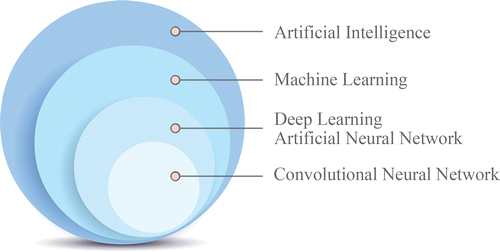
\includegraphics[width=0.45\textwidth]{img/chapters/estado-del-arte/cnn-radiologic.png}
\caption{\label{fig:cnn-dlnn}Las CNN son un subconjunto de redes neuronales de Deep Learning \cite{ankile2020deep}}
\end{figure}

\begin{itemize}
    \item \textbf{Crecimiento de parámetros}. El uso de un perceptron por cada píxel hace que la cantidad de parámetros aumente rápidamente.
    \item \textbf{Traducciones}. Un \gls{mlp} estándar trataría una imagen y su versión ligeramente desplazada como dos imágenes complemente diferentes. Por ejemplo, reconocer un automóvil en una imagen no debería de depender de en qué lugar de la imagen se encuentra.
    \item \textbf{Espacialidad}. Los \gls{mlp} no tienen en cuenta las relaciones espaciales en las imágenes. El hecho de que dos píxeles se encuentren cerca es información significativa.
\end{itemize}

Las \gls{cnn} resuelven el problema de la comprensión de las imágenes, utilizando redes de complejidad más manejable. La red neuronal especial tiene en cuenta que la cercanía entre píxeles tiene significado y que los elementos de interés pueden aparecer en cualquier parte de una imagen. Esto se logra mediante el uso de una operación de convolución lineal. El uso de esta operación en una o más capas es lo que define a una \gls{cnn}. En ocasiones las suposiciones subyacentes a las opciones de diseño de las \gls{cnn} deben disminuirse o alterarse debido a la naturaleza de los datos de entrada. Aunque la complejidad computacional es más manejable, las redes tienden a ser más profundas. Esto crea algoritmos inteligentes para calcular las convoluciones.

La idea principal detrás de la convolución es la identificación de características en los datos de entrada mediante la aplicación de un kernel (también conocido como filtro) en los datos de entrada. Tanto los datos de entrada como el kernel tienen una estructura similar a una cuadrícula y se pueden representar como tensores, que son matrices multidimensionales. El kernel puede ser de cualquier tamaño y, por lo general, es más pequeño que los datos de entrada. Los núcleos se utilizan para identificar características en los datos de entrada, como los bordes de una imagen. Los datos de entrada se convolucionan con el kernel, lo que significa que el kernel se ``desliza'' a través de los datos de entrada, calculando el producto escalar o el producto matricial (según las dimensiones) entre la parte superpuesta de los datos de entrada y el kernel. En la figura \ref{fig:ejemplo-convolucion} se puede ver un ejemplo ilustrativo de la operación de convolución.

\begin{figure}[ht]
\centering
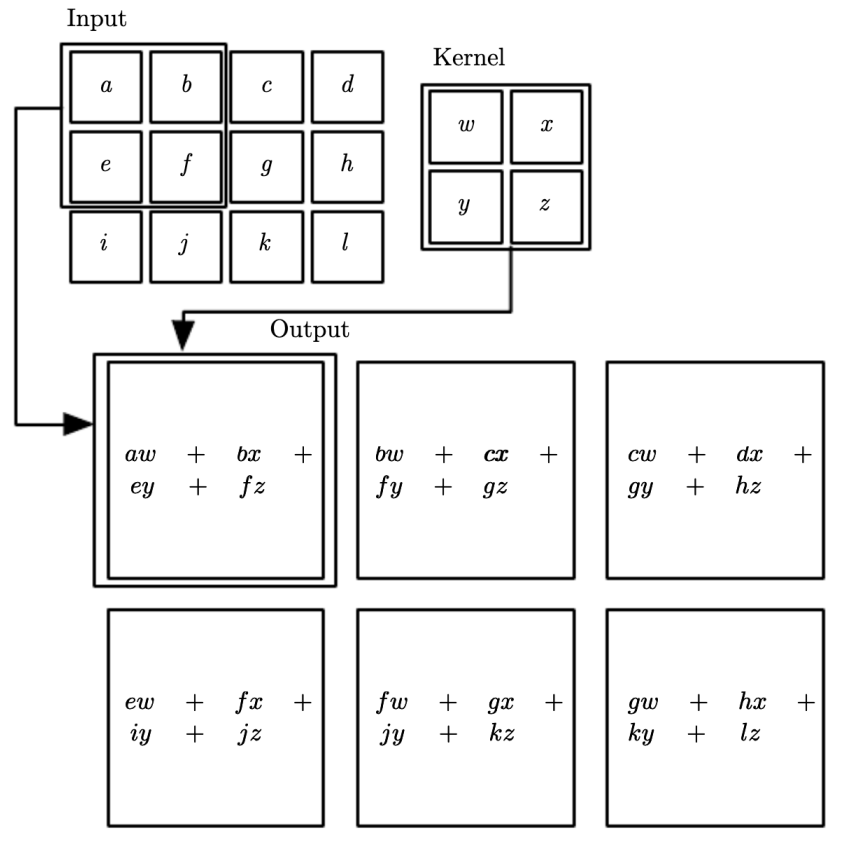
\includegraphics[width=0.4\textwidth]{img/chapters/estado-del-arte/ejemplo-convolucion.png}
\caption{\label{fig:ejemplo-convolucion}Ejemplo de convolución de datos de entrada bidimensionales \cite{ankile2020deep}}
\end{figure}

La operación de convolución se define como:

\begin{equation}
\label{eq:operacion-convolucion1}
s(t) = (x*w)(t) = \int x(a)w(t-a)da
\end{equation}

donde $x$ es la función que se asigna a un valor específico en los datos de entrada y $w$ representa el núcleo. Esta formulación se puede considerar como un promedio de suavizado de $x$ en todo su dominio, dando mayor peso a los valores más cercanos a $t$. Si los valores de entrada son discretos, la operación de convolución se puede reescribir mediante el siguiente sumatorio:

\begin{equation}
\label{eq:operacion-convolucion2}
s(t) = (x*w)(t) = \sum_{a=-\infty}^\infty x(a)w(t-a)
\end{equation}

La entrada suele ser multidimensional. En ese caso, se pueden reemplazar las funciones con funciones multivariables, es decir, operando en tensores. Suponiendo un ejemplo de aplicación de convolución a una imagen bidimensional $I$ como entrada. Luego, se puede usar un kernel $K$ bidimensional, y la operación se puede escribir de la siguiente manera:

\begin{equation}
\label{eq:operacion-convolucion3}
S(i,j) = (I*K)(i,j) = \sum_{m} \sum_{n} I(m,n) K (i - m, j - n)
\end{equation}

Es decir, dado un píxel en la entrada, ubicado en la fila $i$ y la columna $j$, la convolución se calcula colocando el centro del núcleo sobre el píxel de entrada y sumando el producto de los parámetros del núcleo superpuestos y los píxeles de entrada para producir el valor de salida para $i$ y $j$.

\subsection*{Ejemplo de aplicación: Detección de tumores en mamografías}
\label{subsec:ejemplos-aplicacion-cnn}

Una aplicación interesante de las redes neuronales convolucionales se encuentra dentro del campo de la radiología. Cada año, millones de mujeres se someten a un tratamiento para la detección de cánceres en una etapa temprana mediante mamografías. El artículo \cite{mammography2019} muestra que las \gls{cnn} ya pueden detectar cánceres en una etapa temprana con alta precisión. De hecho, su algoritmo ya está superando en muchos aspectos a los medicina estadounidense. El uso de \gls{cnn} en el diagnóstico puede reducir en gran medida el coste para los hospitales, haciendo que las pruebas estén disponibles para un público más amplio y, al mismo tiempo, aumentando la precisión del diagnóstico.

\begin{figure}[ht]
\centering
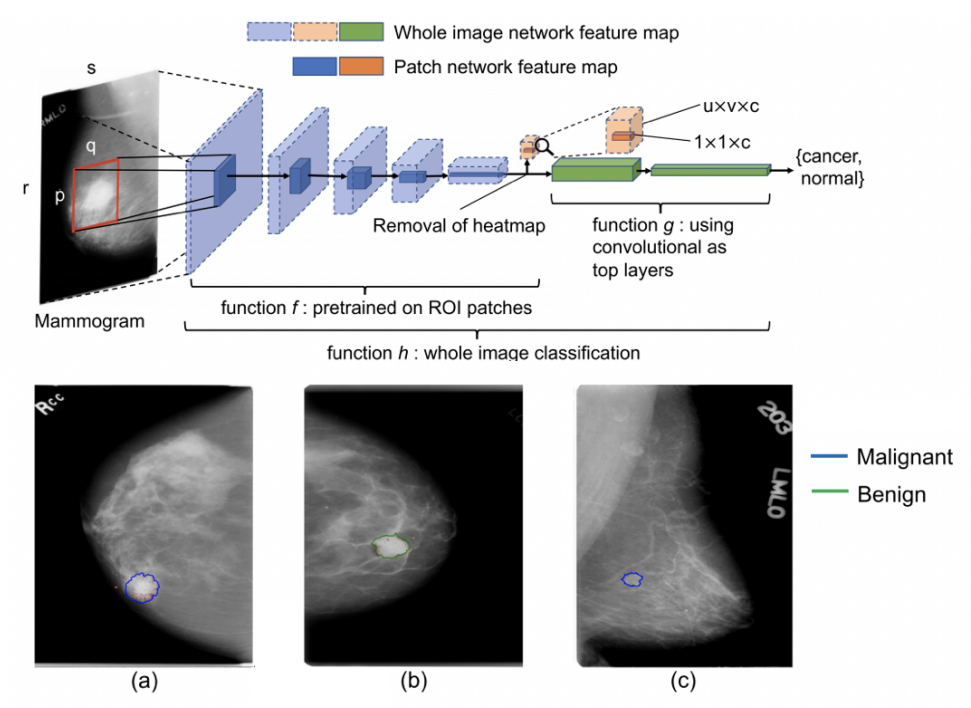
\includegraphics[width=0.55\textwidth]{img/chapters/estado-del-arte/cnn-mamografia.png}
\caption{\label{fig:ejemplo-mamografia}Ejemplo de convolución de datos de entrada bidimensionales \cite{ankile2020deep}}
\end{figure}

La \gls{cnn} resultante se ejecutó en varias bases de datos con un \gls{auc} en las imágenes de menor calidad de 0,91. Entrenando una red con imágenes de alta resolución de la base de datos INbreast \cite{moreira2011}, su mejor modelo logró un \gls{auc} por imagen de 0,95. Combinando todos sus modelos, este número se elevó hasta 0,98 con una sensibilidad del 86,7\% y una especificidad del 96,1\%. Esto muestra que las \gls{cnn} pueden realizar tareas que ahorran costes pero, lo que es más importante, salvan vidas. En base al resultado del artículo \cite{mammography2019}, esto significaría que la \gls{cnn} está superando al personal médico en la detección y clasificación de tumores. Los médicos tienen solo un 0,3\% más de probabilidades de detectar correctamente un tumor maligno, pero tienen un 7,2\% menos de probabilidades de encontrar correctamente que un paciente esté sano.

\section{Algoritmos de detección de objetos}
\label{sec:tecnicas-utilizadas-detection}

En esta sección se va exponer los distintos algoritmos de detección de objetos que están siendo utilizados en los últimos años. Por un lado, están los detectores basados en regiones como Faster \gls{r-cnn}, donde a partir de una imagen de entrada, se proponen múltiples regiones dentro de la imagen a través de un algoritmo de búsqueda selectiva, de donde se obtienen múltiples regiones en base a características de la imagen que proporcionan potenciales zonas que pueden contener objetos. Estas regiones serán con las que se alimentará a la \gls{cnn} para clasificarlas y obtener a la clase que pertenecen. Esto último se consigue a través de \gls{svm}. Por otro lado, están los detectores en tiempo real como \gls{yolo}, \gls{ssd} o EfficientDet donde la red neuronal solo necesita ``mirar'' una vez para predecir los objetos que hay en una imagen.

\subsection{Faster R-CNN}
\label{subsec:faster-rcnn}

Faster \gls{r-cnn} \cite{ren2016faster} es una extensión de Fast \gls{r-cnn} \cite{7410526}. Como su nombre indica, Faster \gls{r-cnn} es más rápido que Fast \gls{r-cnn} gracias a la red de propuesta regional (\gls{rpn}).

La arquitectura de Faster \gls{r-cnn} se muestra en la figura \ref{fig:arquitectura-faster-rcnn}. Consta de 2 módulos:

\begin{itemize}
    \item \gls{rpn}: para generar propuestas regionales.
    \item Fast \gls{r-cnn}: para detectar objetos en las regiones propuestas.
\end{itemize}

El módulo \gls{rpn} es responsable de generar propuestas regionales. Aplica el concepto de atención en redes neuronales, por lo que guía al módulo de detección Fast \gls{r-cnn} hacia dónde buscar objetos en la imagen.

Las capas convolucionales se comparten entre los módulos \gls{rpn} y Fast \gls{r-cnn}.

Faster \gls{r-cnn} funciona de la siguiente manera:

\begin{itemize}
    \item El \gls{rpn} genera propuestas regionales.
    \item Para todas las propuestas de región en la imagen, se extrae un vector de características de longitud fija de cada región utilizando la capa de agrupación de \gls{roi}.
    \item Los vectores de características extraídos luego se clasifican usando Fast \gls{r-cnn}.
    \item Se devuelven las puntuaciones de clase de los objetos detectados además de sus cuadros delimitadores.
\end{itemize}

\begin{figure}[ht]
\centering
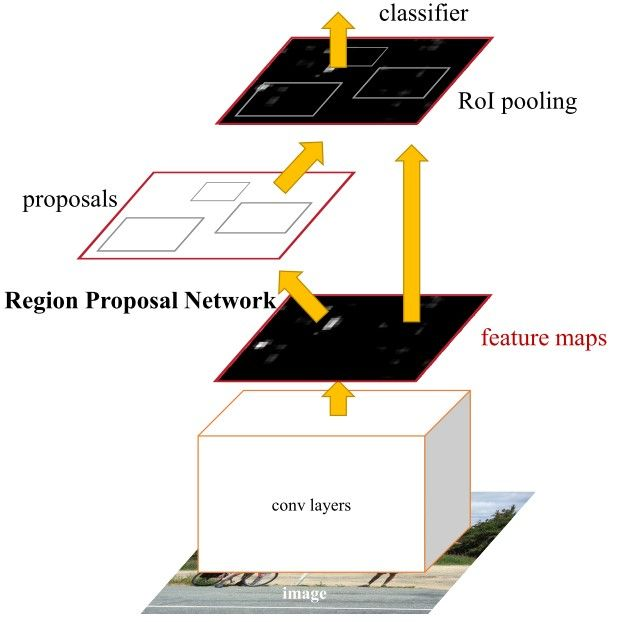
\includegraphics[width=0.45\textwidth]{img/chapters/estado-del-arte/arquitectura-faster-rcnn.jpg}
\caption{\label{fig:arquitectura-faster-rcnn}Arquitectura de Faster R-CNN \cite{ren2016faster}}
\end{figure}

\subsubsection*{Region Proposal Network (RPN)}
\label{subsubsec:region-proposal-network}

Los modelos \gls{r-cnn} y Fast \gls{r-cnn} dependen del algoritmo de búsqueda selectiva para generar propuestas de región. Cada propuesta se envía a una \gls{cnn} previamente capacitada para su clasificación. En \cite{ren2016faster} se propuso una red denominada red de propuestas regionales (\gls{rpn}) que puede producir las propuestas regionales. Esto tiene algunas ventajas:

\begin{enumerate}
    \item Las propuestas de región ahora se generan utilizando una red que podría entrenarse y personalizarse de acuerdo con la tarea de detección.
    \item Debido a que las propuestas se generan utilizando una red, ésta se puede entrenar de un extremo a otro para personalizarla en la tarea de detección. Por lo tanto, produce mejores propuestas de región en comparación con métodos genéricos como Selective Search y EdgeBoxes.
    \item El \gls{rpn} procesa la imagen utilizando las mismas capas convolucionales utilizadas en la red de detección Fast \gls{r-cnn}. Por lo tanto, el \gls{rpn} no necesita más tiempo para producir las propuestas en comparación con los algoritmos como la búsqueda selectiva.
    \item Debido a que comparten las mismas capas convolucionales, el \gls{rpn} y el Fast \gls{r-cnn} se pueden fusionar/unificar en una sola red. Por consiguiente, el entrenamiento se realiza solo una vez.
\end{enumerate}

El \gls{rpn} funciona en el mapa de características de salida devuelto desde la última capa convolucional compartida con Fast \gls{r-cnn}. Esto se muestra en la figura \ref{fig:variacion-anchor-boxes-faster-rcnn}. Sobre la base de una ventana rectangular de tamaño $n*n$, una ventana deslizante atraviesa el mapa de características. Para cada ventana, se generan varias propuestas de regiones candidatas. Estas propuestas no son las propuestas finales, ya que se filtrarán en función de su ``puntuación de objetividad''.

\subsubsection*{Anchor}
\label{subsubsec:anchor-faster-rcnn}

Como se puede ver en la figura \ref{fig:variacion-anchor-boxes-faster-rcnn}, el mapa de características de la última capa de convolución compartida se pasa a través de una ventana deslizante rectangular de tamaño $n*n$, donde $n = 3$ para la red VGG-16. Para cada ventana, se generan propuestas de región $K$. Cada propuesta se parametriza según un cuadro de referencia que se denomina \textit{anchor box}. Los 2 parámetros de los anchor boxes son:

\begin{enumerate}
    \item Escala.
    \item Relación de aspecto.
\end{enumerate}

Generalmente, hay 3 escalas y 3 relaciones de aspecto y, por lo tanto, hay un total de $K = 9$ casillas de anclaje. Pero $K$ puede ser diferente de 9. En otras palabras, las $K$ regiones se producen a partir de cada propuesta de región, donde cada una de las $K$ regiones varía en la escala o en la relación de aspecto. Algunas de las variaciones del anchor se muestran en la figura \ref{fig:variacion-anchor-boxes-faster-rcnn}.

\begin{figure}[ht]
\centering
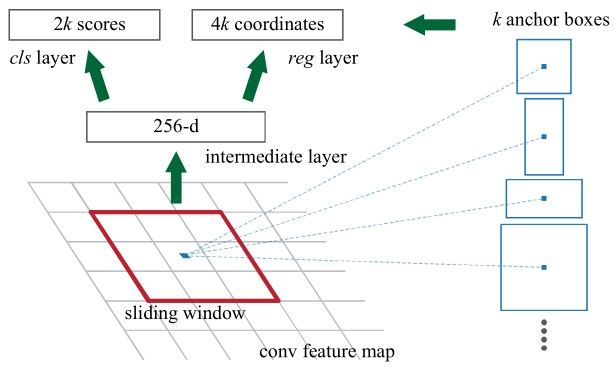
\includegraphics[width=0.45\textwidth]{img/chapters/estado-del-arte/variacion-anchor-boxes-faster-rcnn.jpg}
\caption{\label{fig:variacion-anchor-boxes-faster-rcnn}Variación de los anchor boxes Faster R-CNN \cite{ren2016faster}}
\end{figure}

Utilizando anclajes de referencia (anchor boxes), se utiliza una sola imagen a una sola escala y, al mismo tiempo, se pueden ofrecer detectores de objetos invariantes en escala, ya que los anclajes existen a diferentes escalas. Esto evita el uso de múltiples imágenes o filtros. Los anclajes de múltiples escalas son clave para compartir características en el \gls{rpn} y la red de detección Fast \gls{r-cnn}.

Para cada propuesta de región $n*n$, se extrae un vector de características (de longitud 256 para la red ZF y 512 para la red VGG-16). Este vector luego se alimenta a 2 capas hermanas completamente conectadas:

\begin{enumerate}
    \item La primera capa \gls{fc} se llama \texttt{cls} y representa un clasificador binario que genera la puntuación de objetividad para cada propuesta de región (es decir, si la región contiene un objeto o es parte del fondo).
    \item La segunda capa \gls{fc} se llama \texttt{reg}, que devuelve un vector 4-D que define el cuadro delimitador de la región.
\end{enumerate}

La primera capa \gls{fc} (es decir, clasificador binario) tiene 2 salidas. El primero es para clasificar la región como fondo y el segundo es para clasificar la región como un objeto. La siguiente sección analiza cómo se asigna la puntuación de objetividad a cada anchor box y cómo se utiliza para producir la etiqueta de clasificación.

\subsection{SSD: Single Shot MultiBox Detector}
\label{subsec:ssd}

\gls{ssd} \cite{Liu_2016} es un modelo de detección de objetos en imágenes empleando únicamente una \gls{dnn}. \gls{ssd} discretiza el espacio de salida de los cuadros delimitadores en un conjunto de cuadros predeterminados en diferentes proporciones y escalas por ubicación del mapa de características. En el momento de la predicción, la red genera puntuaciones para la presencia de cada categoría de objeto en cada cuadro predeterminado y produce ajustes en el cuadro para que coincida mejor con la forma del objeto. Además, la red combina predicciones de múltiples mapas de características con diferentes resoluciones para manejar de forma natural objetos de varios tamaños.

\gls{ssd} tiene dos componentes: un modelo backbone y un \gls{ssd} head. El modelo backbone suele ser una red de clasificación de imágenes previamente entrenadas como extractor de características. Típicamente suele ser una red como ResNet entrenada en ImageNet \cite{russakovsky2015imagenet} de la que se ha eliminado la capa de clasificación final \gls{fc}. Por tanto, nos quedamos con una \gls{dnn} que es capaz de extraer el significado semántico de la imagen de entrada al tiempo que conserva la estructura espacial de la imagen, aunque con una resolución más baja. Para ResNet34, el backbone da como resultado un mapa de características de 256 7x7 para una imagen de entrada. El \gls{ssd} head es solo una o varias capas convolucionales agregadas a este backbone y las salidas se interpretan como los cuadros delimitadores y las clases de objetos en la ubicación espacial de las activaciones de las capas finales.

En la figura \ref{fig:ssd-structure}, las primeras capas (cuadros blancos) son el backbone, las últimas capas (cuadros azules) representan el SSD head.

\begin{figure}[ht]
\centering
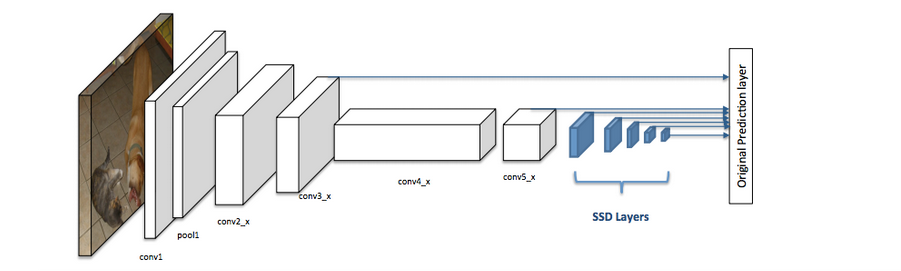
\includegraphics[width=1\textwidth]{img/chapters/estado-del-arte/ssd-structure.png}
\caption{\label{fig:ssd-structure}Arquitectura de una red neuronal convolucional con un detector SSD \cite{how-works-ssd}}
\end{figure}

\subsubsection*{Grid cell}
\label{subsubsec:grid-cell-ssd}

En lugar de usar una ventana deslizante, \gls{ssd} divide la imagen usando una cuadrícula y cada celda de la cuadrícula es responsable de detectar objetos en esa región de la imagen. La detección de objetos simplemente significa predecir la clase y ubicación de un objeto dentro de esa región. Si no hay ningún objeto presente, se considera como la clase de fondo y se ignora la ubicación. Por ejemplo, como se puede observar en la figura usar una cuadrícula de 4x4 en el siguiente ejemplo. Cada celda de la cuadrícula puede mostrar la posición y la forma del objeto que contiene.

\begin{figure}[ht]
\centering
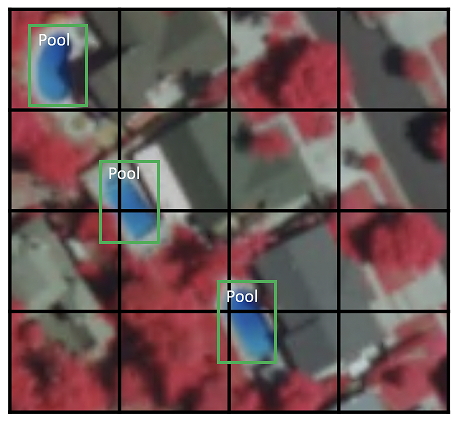
\includegraphics[width=0.3\textwidth]{img/chapters/estado-del-arte/gridcell.png}
\caption{\label{fig:ejemplo-grid-cell}Ejemplo de una cuadrícula 4x4 \cite{how-works-ssd}}
\end{figure}

\subsubsection*{Anchor box}
\label{subsubsec:anchor-box-ssd}

Cada grid cell en \gls{ssd} se puede asignar con múltiples anchor boxes. Estos anchor boxes están predefinidos y cada uno es responsable de un tamaño y forma dentro de una grid cell. Por ejemplo, la piscina de la imagen siguiente corresponde a la anchor box más alta, mientras que el edificio corresponde a la anchor box más ancha.

\begin{figure}[ht]
\centering
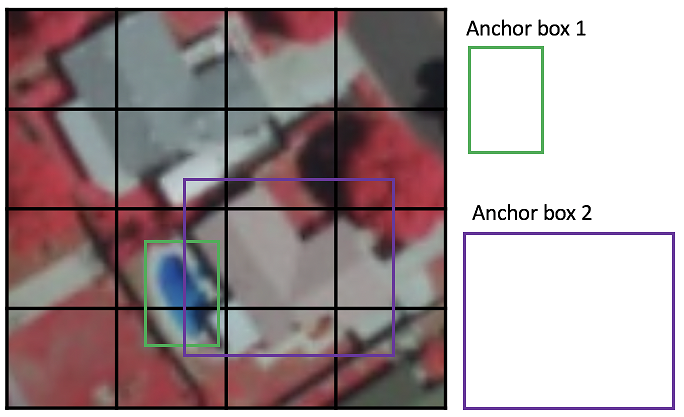
\includegraphics[width=0.45\textwidth]{img/chapters/estado-del-arte/ejemplo-2-anchor-boxes.png}
\caption{\label{fig:ejemplo-2-anchor-boxes}Ejemplo con 2 anchor boxes \cite{how-works-ssd}}
\end{figure}

\gls{ssd} usa una fase de coincidencia durante el entrenamiento, para hacer coincidir el anchor box apropiado con los cuadros delimitadores de cada objeto de ground truth dentro de una imagen. Básicamente, el anchor box con el mayor grado de superposición con un objeto es responsable de predecir la clase de ese objeto y su ubicación. Esta propiedad se utiliza para entrenar la red y para predecir los objetos detectados y sus ubicaciones una vez que la red ha sido entrenada. En la práctica, cada anchor box se especifica mediante una relación de aspecto y un nivel de zoom.

\subsubsection*{Relación de aspecto}
\label{subsubsec:aspect-ratio-ssd}

No todos los objetos tienen forma cuadrada. Algunos son más largos y otros más anchos, en diversos grados. La arquitectura \gls{ssd} permite relaciones de aspecto predefinidas de los anchor boxes para tener en cuenta esto. El parámetro de proporciones se puede utilizar para especificar las diferentes proporciones de los cuadros de anclaje asociados con cada celda de la cuadrícula en cada nivel de zoom/escala.

\begin{figure}[ht]
\centering
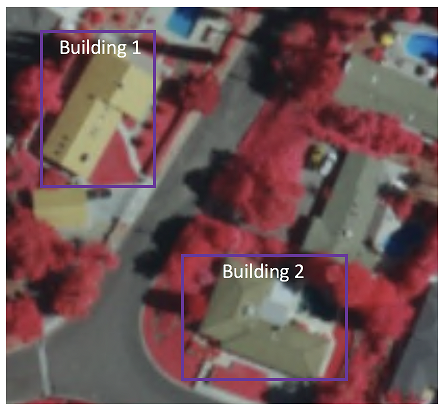
\includegraphics[width=0.30\textwidth]{img/chapters/estado-del-arte/aspect_ratio-ejemplo-ssd.png}
\caption{\label{fig:aspect_ratio-ejemplo-ssd}El cuadro delimitador del edificio 1 es más alto, mientras que el cuadro delimitador del edificio 2 es más ancho \cite{how-works-ssd}}
\end{figure}

\subsubsection*{Nivel de zoom}
\label{subsubsec:zoom-level-ssd}

No es necesario que los anchor boxes tengan el mismo tamaño que la grid cell. Podríamos estar interesados en encontrar objetos más pequeños o más grandes dentro de una celda de la cuadrícula. El parámetro de zoom se utiliza para especificar cuánto deben ampliarse o reducirse los cuadros de anclaje con respecto a cada celda de la cuadrícula. Al igual que lo que hemos visto en el ejemplo de el anchor box, el tamaño del edificio es generalmente más grande que la piscina.

\subsubsection*{Campo receptivo}
\label{subsubsec:receptive-field-ssd}

El campo receptivo se define como la región en el espacio de entrada que está mirando una función de \gls{cnn} en particular, es decir, que se ve afectada. Debido a la operación de convolución, las características en diferentes capas representan diferentes tamaños de región en la imagen de entrada. A medida que se profundiza, el tamaño representado por una característica aumenta. En este ejemplo que se puede observar en la figura \ref{fig:receptive-field-ssd}, se comienza con la capa inferior (5x5) y luego se aplica una convolución que da como resultado la capa intermedia (3x3) donde una característica (píxel verde) representa una región de 3x3 de la capa de entrada (capa inferior). Después se aplica la convolución a la capa intermedia y se obtiene la capa superior (2x2) donde cada característica corresponde a una región de 7x7 en la imagen de entrada. Este tipo de matriz 2D verde y naranja también se denomina mapa de características, que se refieren a un conjunto de características creadas al aplicar el mismo extractor de características en diferentes ubicaciones del mapa de entrada en una ventana deslizante. Las características del mismo mapa de características tienen el mismo campo receptivo y buscan el mismo patrón pero en diferentes ubicaciones. Esto crea la invariancia espacial de ConvNet.

El campo receptivo es la premisa central de la arquitectura \gls{ssd}, ya que permite detectar objetos a diferentes escalas y generar un cuadro delimitador más ajustado. El backbone ResNet34 genera mapas de características de 256 7x7 para una imagen de entrada. Si especificamos una cuadrícula de 4x4, el enfoque más simple es sencillamente aplicar una convolución a este mapa de características y convertirlo a 4x4. Este enfoque puede funcionar hasta cierto punto y es exactamente la idea de \gls{yolo}. El paso extra dado por \gls{ssd} es que aplica más capas convolucionales al mapa de características del backbone y hace que cada una de estas capas de convolución genere resultados de detección de objetos. Como las capas anteriores que tienen un campo receptivo más pequeño pueden representar objetos de menor tamaño, las predicciones de las capas anteriores ayudan a tratar con objetos de menor tamaño.

Debido a esto, \gls{ssd} permite definir una jerarquía de celdas de cuadrícula en diferentes capas. Por ejemplo, se podría usar una cuadrícula de 4x4 para encontrar objetos más pequeños, una cuadrícula de 2x2 para encontrar objetos de tamaño medio y una cuadrícula de 1x1 para encontrar objetos que cubran toda la imagen.

\begin{figure}[ht]
\centering
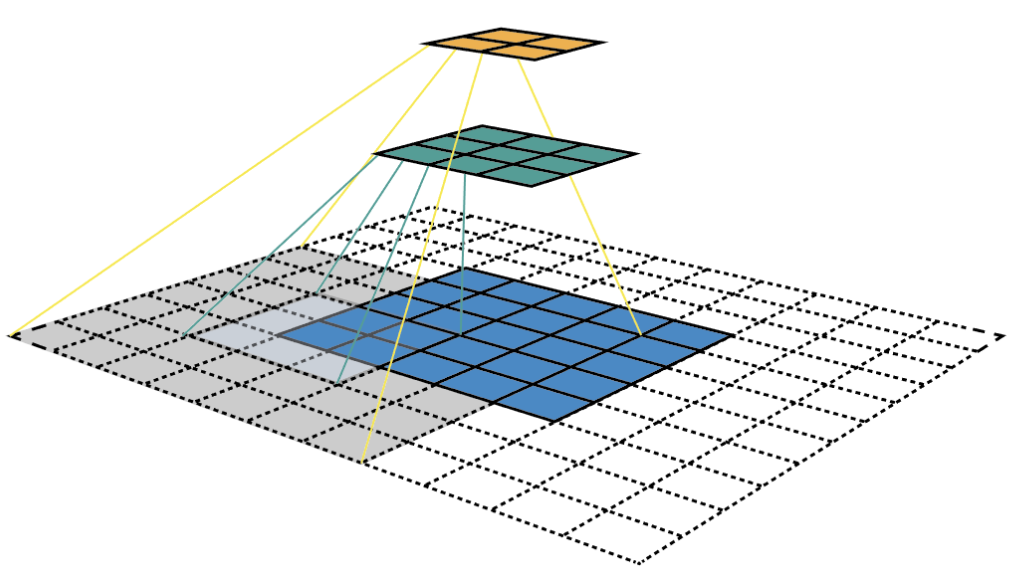
\includegraphics[width=0.4\textwidth]{img/chapters/estado-del-arte/receptive-field.png}
\caption{\label{fig:receptive-field-ssd}Visualización de mapas de características de CNN y campo receptivo \cite{how-works-ssd}}
\end{figure}

\subsection{EfficientDet}
\label{subsec:efficientdet}

EfficientDet \cite{tan2020efficientdet} se trata de un detector de objetos escalable y eficiente. Sobre la base del trabajo que se realizó anterior sobre el escalado de redes neuronales se logra una alta precisión y es hasta 9 veces más pequeño y usa significativamente menos cálculos en comparación con los detectores del Estado del Arte. En la figura \ref{fig:arquitectura-efficientdet} se muestra la arquitectura de red general de los modelos.

EfficientDet surge en noviembre de 2019 con la necesidad de aplicar soluciones en la mejora de la eficiencia computacional mediante la realización de un estudio sistemático de modelos de detección de última generación. Como ya se vio en la sección \ref{subsec:ssd}, los detectores de objetos tienen tres componentes principales: un backbone que extrae características de una imagen dada, una red de características que toma múltiples niveles de características de la red troncal como entrada y genera una lista de características fusionadas que representan características de la imagen y una red final que usa las características fusionadas para predecir la clase y ubicación de cada objeto. Al examinar las opciones de diseño para estos componentes, EfficientDet identifica varias optimizaciones clave para mejorar el rendimiento y la eficiencia.

\begin{figure}[ht]
\centering
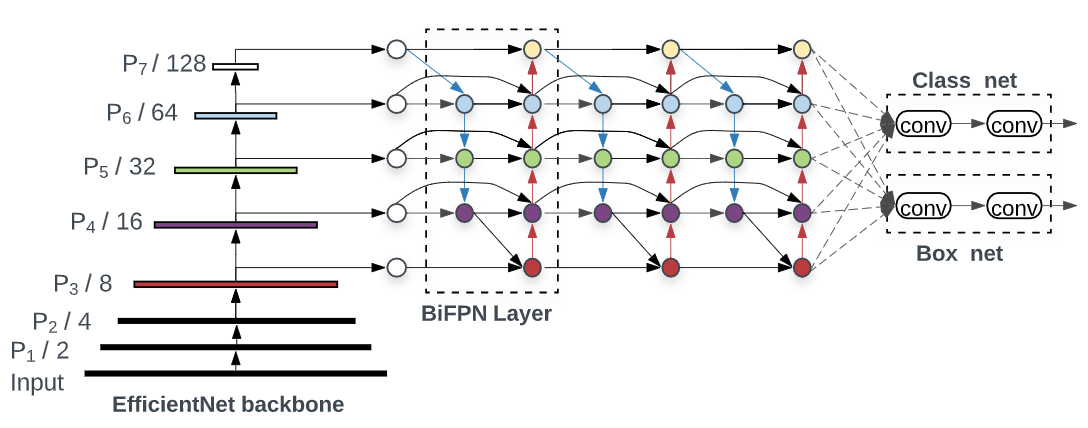
\includegraphics[width=0.7\textwidth]{img/chapters/estado-del-arte/arquitectura-efficientdet.png}
\caption{\label{fig:arquitectura-efficientdet}Arquitectura de EfficientDet \cite{tan2020efficientdet}}
\end{figure}

Los detectores de objetos anteriores se basan principalmente en ResNet, ResNeXt o AmoebaNet como backbones, que son menos potentes o tienen menor eficiencia que la de EfficientNet. Al implementar primero un backbone EfficientNet, es posible lograr una eficiencia mucho mayor. Por ejemplo, a partir de una RetinaNet que emplea el backbone ResNet-50, se puede observar que simplemente reemplazar ResNet-50 con EfficientNet-B3 puede mejorar la precisión en un 3\% y reducir los cálculos en un 20\%.

Otra optimización es mejorar la eficiencia de las redes de características. Si bien la mayoría de los detectores anteriores simplemente emplean una \gls{fpn}, se puede observar que el \gls{fpn} de arriba hacia abajo está inherentemente limitado por el flujo de información unidireccional. Los \gls{fpn} alternativos, como PANet, agregan un flujo ascendente adicional a costa de más cálculos. Los esfuerzos para aprovechar la \gls{nas} descubrieron la arquitectura \gls{nas}-\gls{fpn} más compleja. Sin embargo, si bien esta estructura de red es efectiva, también es irregular y altamente optimizada para una tarea específica, lo que dificulta la adaptación a otras tareas.

Para abordar estos problemas, EfficientDet presenta una nueva red de funciones bidireccionales, Bi\gls{fpn}, que incorpora la idea de fusión de funciones multinivel de \gls{fpn}/PANet /\gls{nas}-\gls{fpn} que permite que la información fluya tanto en la dirección de arriba hacia abajo como de abajo hacia arriba, mientras utiliza conexiones regulares y eficientes.

\begin{figure}[ht]
\centering
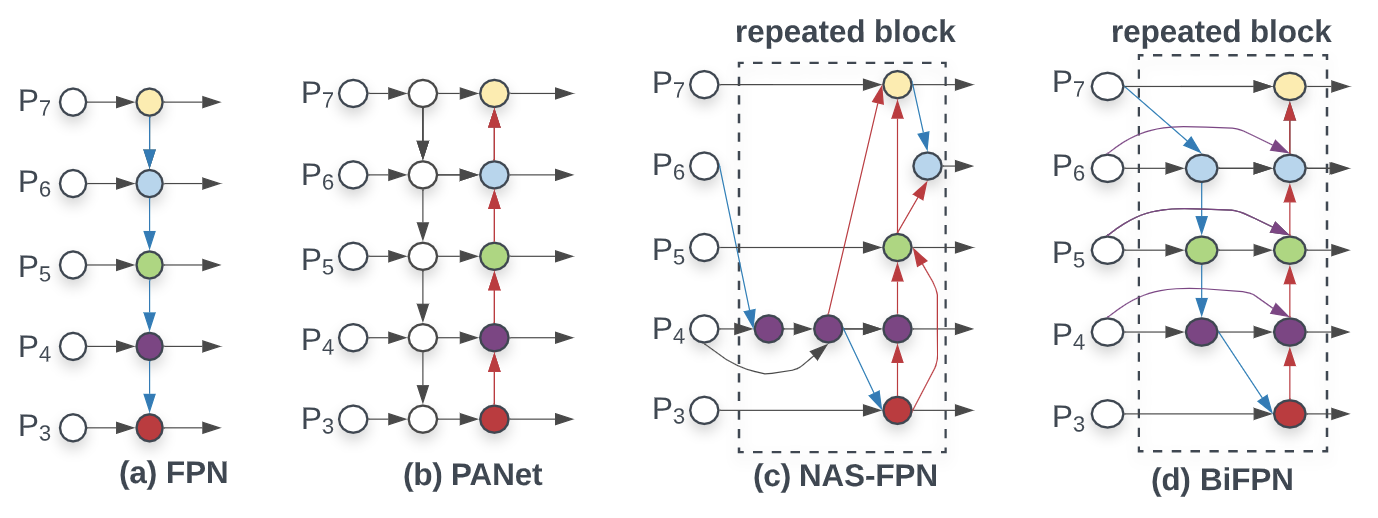
\includegraphics[width=0.7\textwidth]{img/chapters/estado-del-arte/comparativa_fpn+panet+nas-fpn+bifpn.png}
\caption{\label{fig:comparativa-bifpn}Comparativa entre biFPN y las demás redes de características previas \cite{tan2020efficientdet}}
\end{figure}

Para mejorar aún más la eficiencia, EfficientDet plantea una nueva técnica de fusión rápida normalizada. Las propuestas tradicionales generalmente tratan todas las características de entrada al \gls{fpn} por igual, incluso aquellas con diferentes resoluciones. Sin embargo, se observa que las características de entrada en diferentes resoluciones a menudo tienen contribuciones desiguales a las características de salida. Por lo tanto, agregando un peso adicional para cada característica de entrada se permite que la red aprenda la importancia de cada una. EfficientDet también propone reemplazar todas las circunvoluciones regulares con circunvoluciones separables en profundidad menos costosas. Con estas optimizaciones, Bi\gls{fpn} mejora aún más la precisión en un 4\%, al tiempo que reduce el coste de cálculo en un 50\%.

Una tercera optimización implica lograr mejores compensaciones de precisión y eficiencia bajo diferentes limitaciones de recursos. Escalar conjuntamente la profundidad, el ancho y la resolución de una red puede mejorar significativamente la eficiencia del reconocimiento de imágenes. EfficientDet ofrece un nuevo método de escalado compuesto para detectores de objetos, que escala conjuntamente la resolución/profundidad/ancho. Cada componente de la red, es decir, el backbone, la característica y la red de predicción de cuadro/clase, tendrá un único factor de escala compuesto que controla todas las dimensiones de escala utilizando reglas basadas en heurísticas. Este enfoque permite determinar fácilmente cómo escalar el modelo calculando el factor de escala para las restricciones de recursos de destino dadas.

Combinando el nuevo backbone y Bi\gls{fpn}, surge una línea de base EfficientDet-D0 de tamaño pequeño y aplicando una escala compuesta para obtener de EfficientDet-D1 a D7. Cada modelo consecutivo tiene un coste computacional más alto, que cubre una amplia gama de restricciones de recursos desde 3 mil millones de \gls{flops} hasta 300 mil millones de \gls{flops}, proporcionando una mayor precisión.

\subsection{YOLOv4}
\label{subsec:yolov4}

\gls{yolo} \cite{bochkovskiy2020yolov4} es uno de los algoritmos de detección de objetos más eficientes que existen. La primera versión fue publicada por Joseph Redmon \cite{redmon2016look} en 2016 y la implementación más reciente \cite{bochkovskiy2020yolov4} está liderada por Alexey Bochkovsky. Predice tanto la posición (representada como un cuadro delimitador) como la clasificación de objetos en imágenes.

\gls{yolo} tiene como objetivo encontrar las siguientes variables en una imagen:

\begin{itemize}
    \item $(bx, by)$ - el centro de un cuadro delimitador.
    \item $(bw, bh)$ - el ancho y alto de un cuadro delimitador.
    \item $c$ - la clase del objeto.
    \item $P_c$ - la probabilidad de que haya un objeto de clase $c$ en el cuadro.
\end{itemize}

\gls{yolo} divide la imagen en una imagen de 19x19, donde cada celda predice 5 cuadros delimitadores de la forma $y = (Pc, bx, by, bw, bh, c)$. Esto da $19x19x5 = 1.805$ cuadros delimitadores diferentes por imagen. La eliminación de las cajas con un $Pc$ bajo se denomina \textit{non-max suppression}.

La principal diferencia entre \gls{yolov4} y las implementaciones anteriores es el enfoque en la velocidad. El objetivo del nuevo algoritmo \gls{yolo} es que cualquier persona que disponga de una \gls{gpu} de alta gama pueda aplicar el algoritmo para lograr una alta precisión para el reconocimiento de imágenes ejecutándose en tiempo real. En la figura \ref{fig:yolov4-speed-accuracy-vs-others}, se muestran los resultados de la comparación entre \gls{yolov4} y otras arquitecturas, donde es evidente que \gls{yolov4} supera a la mayoría de las otras redes neuronales en términos de precisión promedio y lo hace a más del doble de la velocidad de fotogramas. Esto diferencia mucho a \gls{yolov4} de los otros algoritmos, ya que se puede utilizar en la clasificación de objetos en tiempo real con una precisión casi humana. Por ejemplo, la \gls{cnn} puede diferenciar entre automóviles, bicicletas y camiones que circulan por una carretera. Con su alta velocidad y precisión sorprendentemente buena, \gls{yolo} es ampliamente adoptado y, como tal, es un éxito.

\begin{figure}[ht]
\centering
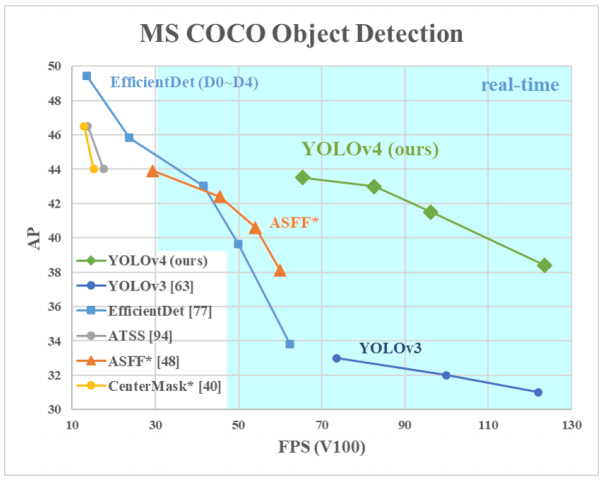
\includegraphics[width=0.5\textwidth]{img/chapters/estado-del-arte/yolov4-vs-others.png}
\caption{\label{fig:yolov4-speed-accuracy-vs-others}Comparativa velocidad y precisión de YOLOv4 frente a otras arquitecturas \cite{bochkovskiy2020yolov4}}
\end{figure}

\subsubsection*{Estructura de un detector de objetos}
\label{subsubsec:estructura-detector-objetos}

Todos los detectores de objetos toman una imagen como entrada y comprimen las características a través de una red neuronal convolucional. En la clasificación de imágenes, estos backbones son el final de la red y se pueden hacer predicciones a partir de ellas. En la detección de objetos, es necesario dibujar varios cuadros delimitadores alrededor de las imágenes junto con la clasificación, por lo que las capas de características convolucional del backbone deben mezclarse unas de otras. La combinación de capas de características del backbone ocurre en el neck.

También es útil dividir los detectores de objetos en dos categorías: detectores de una etapa y detectores de dos etapas. La detección ocurre en el head. Los detectores de dos etapas desacoplan la tarea de localización y clasificación de objetos para cada cuadro delimitador. Los detectores de una etapa hacen las predicciones para la localización y clasificación de objetos al mismo tiempo. \gls{yolo} es un detector de una etapa, por lo tanto, solo mira una vez (You Only Look Once).

\begin{figure}[ht]
\centering
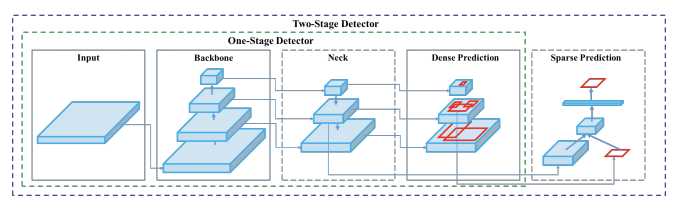
\includegraphics[width=0.75\textwidth]{img/chapters/estado-del-arte/one-two-stage-detector.png}
\caption{\label{fig:one-two-stage-detector}Arquitectura de detectores de objetos de una y dos etapas \cite{bochkovskiy2020yolov4}}
\end{figure}

\subsubsection*{Backbone de YOLOv4}
\label{subsubsec:yolov4-backbone}

El backbone de la red de un detector de objetos típicamente suele estar pre-entrenada en la clasificación de ImageNet \cite{russakovsky2015imagenet}. El entrenamiento previo significa que los pesos de la red ya se han adaptado para identificar características relevantes en una imagen, aunque se modificarán en la nueva tarea de detección de objetos.

Los autores consideraron los siguientes backbones para el detector de objetos \gls{yolov4}:

\begin{itemize}
    \item CSPResNext50.
    \item CSPDarknet53.
    \item EfficientNet-B3.
\end{itemize}

CSPResNext50 y CSPDarknet53 se basan en DenseNet. DenseNet fue diseñado para conectar capas en redes neuronales convolucionales con los siguientes objetivos: aliviar el problema del gradiente de desaparición (es difícil retropropulsar señales de pérdida a través de una red muy profunda), reforzar la propagación de características, alentar a la red a reutilizar características y reducir el número de parámetros de red.

En CSPResNext50 y CSPDarknet53, DenseNet se ha editado para separar el mapa de características de la capa base copiándolo y enviando una copia a través del bloque denso y enviando otra directamente a la siguiente etapa. La idea con CSPResNext50 y CSPDarknet53 es eliminar los cuellos de botella computacionales en DenseNet y mejorar el aprendizaje al pasar una versión sin editar del mapa de características.

EfficientNet fue diseñado por Google Brain para estudiar principalmente el problema de escala de las redes neuronales convolucionales. Hay muchas decisiones que puede tomar al escalar su ConvNet, incluido el tamaño de entrada, la escala de ancho, la escala de profundidad y la escala de todo lo anterior. El artículo \cite{tan2020efficientdet} postula que hay un punto óptimo para todos estos y, a través de la búsqueda, lo encuentran.

EfficientNet supera a las otras redes de tamaño comparable en clasificación de imágenes. Los autores de \gls{yolov4} postulan, sin embargo, que las otras redes pueden funcionar mejor en la configuración de detección de objetos y decidieron experimentar con todas ellas.

En base a los resultados experimentales, la red \gls{yolov4} final implementa CSPDarknet53 para el backbone.

\subsubsection*{Neck de YOLOv4}
\label{subsubsec:yolov4-neck}

El siguiente paso en la detección de objetos es mezclar y combinar las características formadas en el backbone de ConvNet para prepararse para el paso de detección. \gls{yolov4} considera algunas opciones para el neck que incluyen: \gls{fpn}, \gls{pan}, \gls{nas}-\gls{fpn}, Bi\gls{fpn}, \gls{asff} y \gls{sfam}.


Los componentes del neck normalmente fluyen hacia arriba y hacia abajo entre las capas y conectan solo las pocas capas al final de la red convolucional.

Como se pudo observar en la figura \ref{fig:comparativa-bifpn}, EfficientDet utiliza la búsqueda de arquitectura neuronal para encontrar la mejor forma de bloques en la parte del neck de la red, llegando a \gls{nas}-\gls{fpn}. Los autores de EfficientDet lo modificaron ligeramente para hacer que la arquitectura sea más intuitiva (y probablemente funcione mejor en sus conjuntos de desarrollo).

\gls{yolov4} elige \gls{pan}et para la agregación de funciones de la red. No hay escrito mucho sobre el fundamento de esta decisión, y dado que \gls{nas}-\gls{fpn} y Bi\gls{fpn} se escribieron al mismo tiempo, se prevé que sea un área de investigación futura.

Además, \gls{yolov4} agrega un bloque \gls{spp} después de CSPDarknet53 para aumentar el campo receptivo y separar las características más importantes del backbone.

\subsubsection*{Head de YOLOv4}
\label{subsubsec:yolov4-head}

\gls{yolov4} implementa el mismo head \gls{yolo} que \gls{yolo}v3 \cite{redmon2018yolov3} para la detección con el anchor basado en pasos de detección y tres niveles de granularidad de detección.

\subsection{Comparativa de los diferentes detectores}
\label{subsec:comparativa-detectores}

En esta sección se va a evaluar cuantitativamente las principales métricas de los detectores de objetos que se han expuesto anteriormente. Estas métricas, junto a otras muy importantes en la evaluación de modelos entrenados en las distintas arquitecturas, se explicarán con más detalle en la sección \ref{subsec:metricas-calidad}.

Las métricas que se recogen en las siguientes tablas han sido obtenidas en base al dataset \gls{coco}, un conjunto de datos de referencia que se emplea para la evaluar el rendimiento de los modelos de visión por computadora de última generación. Este dataset se describirá con mayor detalle en la sección \ref{subsec:coco-dataset}.

En la tabla \ref{tab:maxwell-speed-accuracy} se muestran los resultados obtenidos en los detectores \gls{yolov4} y \gls{ssd} utilizando \gls{gpu}'s NVIDIA Maxwell.

Como se puede observar, \gls{yolov4} obtuvo un AP50 o \gls{map} de 64,9\% a 31 \gls{fps} frente a un 48,5\% a 22 \gls{fps} que logró \gls{ssd}. Cabe destacar que se están comparando ambos detectores a partir de un tamaño de imágenes de la capa de entrada a la red de 512x512. En términos de velocidad y precisión, \gls{yolov4} se posiciona por encima.

\begin{table}[ht]
\centering
\caption{Velocidad y precisión YOLOv4 y SSD con Maxwell GPU: GTX Titan X (Maxwell) o Tesla M40 GPU \cite{bochkovskiy2020yolov4} \cite{Liu_2016}}
\label{tab:maxwell-speed-accuracy}
\begin{tabular}{llcccc}
\hline
\textbf{Method} & \textbf{Backbone}      & \textbf{Size} & \textbf{FPS}    & \textbf{AP}     & \textbf{AP50}   \\ \hline
YOLOv4          & CSPDarknet-53          & 416           & 38 (M)          & 41,2\%          & 62,8\%          \\
\textbf{YOLOv4} & \textbf{CSPDarknet-53} & \textbf{512}  & \textbf{31 (M)} & \textbf{43,0\%} & \textbf{64,9\%} \\
YOLOv4          & CSPDarknet-53          & 608           & 23 (M)          & 43,5\%          & 65,7\%          \\
                &                        &               &                 &                 &                 \\
SSD             & VGG-16                 & 300           & 43 (M)          & 25,1\%          & 43,1\%          \\
\textbf{SSD}    & \textbf{VGG-16}        & \textbf{512}  & \textbf{22 (M)} & \textbf{28,8\%} & \textbf{48,5\%} \\ \hline
\end{tabular}
\end{table}

En la tabla \ref{tab:pascal-speed-accuracy} se muestran los resultados obtenidos en los detectores \gls{yolov4} y Faster \gls{r-cnn} utilizando \gls{gpu}'s NVIDIA Pascal.

Como se puede observar, \gls{yolov4} obtuvo un AP50 o \gls{map} de 62,8\% a 54 \gls{fps} frente a un 59,2\% a 9,4 \gls{fps} que logró Faster \gls{r-cnn}. El tamaño de las imágenes de capa de entrada a la red de Faster \gls{r-cnn} no se especificó en el benchmark, por lo que se ha comparado con el tamaño más pequeño con el que se realizó la evaluación en \gls{yolov4}, es decir, 416x416. En términos de velocidad y precisión, \gls{yolov4} se posiciona por encima. 

\begin{table}[ht]
\centering
\caption{Velocidad y precisión YOLOv4 y Faster R-CNN con Pascal GPU: Titan X (Pascal), Titan Xp, GTX 1080 Ti, o Tesla P100 GPU \cite{bochkovskiy2020yolov4} \cite{ren2016faster}}
\label{tab:pascal-speed-accuracy}
\begin{tabular}{llcccc}
\hline
\textbf{Method}       & \textbf{Backbone}      & \textbf{Size} & \textbf{FPS}     & \textbf{AP}     & \textbf{AP50}   \\ \hline
\textbf{YOLOv4}       & \textbf{CSPDarknet-53} & \textbf{416}  & \textbf{54 (P)}  & \textbf{41,2\%} & \textbf{62,8\%} \\
YOLOv4                & CSPDarknet-53          & 512           & 43 (P)           & 43,0\%          & 64,9\%          \\
YOLOv4                & CSPDarknet-53          & 608           & 33 (P)           & 43,5\%          & 65,7\%          \\
                      &                        &               &                  &                 &                 \\
\textbf{Faster R-CNN} & \textbf{ResNet-50}     & \textbf{—}    & \textbf{9,4 (P)} & \textbf{39,8\%} & \textbf{59,2\%} \\ \hline
\end{tabular}
\end{table}

En la tabla \ref{tab:volta-speed-accuracy} se muestran los resultados obtenidos en los detectores \gls{yolov4} y EfficientDet utilizando \gls{gpu}'s NVIDIA Volta.

Como se puede observar, \gls{yolov4} obtuvo un AP50 o \gls{map} de 64,9\% a 83 \gls{fps} frente a un 52,2\% a 62,5 \gls{fps} que logró EfficientDet. Cabe destacar que se están comparando ambos detectores a partir de un tamaño de imágenes de la capa de entrada a la red de 512x512. En términos de velocidad y precisión, \gls{yolov4} se posiciona por encima.

\begin{table}[ht]
\centering
\caption{Velocidad y precisión YOLOv4 y EfficientDet con Volta GPU: Titan Volta or Tesla V100 GPU \cite{bochkovskiy2020yolov4} \cite{tan2020efficientdet}}
\label{tab:volta-speed-accuracy}
\begin{tabular}{llcccc}
\hline
\textbf{Method}          & \textbf{Backbone}      & \textbf{Size}        & \textbf{FPS}         & \textbf{AP}          & \textbf{AP50}        \\ \hline
YOLOv4                   & CSPDarknet-53          & 416                  & 96 (V)               & 41,2\%               & 62,8\%               \\
\textbf{YOLOv4}          & \textbf{CSPDarknet-53} & \textbf{512}         & \textbf{83 (V)}      & \textbf{43,0\%}      & \textbf{64,9\%}      \\
YOLOv4                   & CSPDarknet-53          & 608                  & 62 (V)               & 43,5\%               & 65,7\%               \\
                         &                        & \multicolumn{1}{l}{} & \multicolumn{1}{l}{} & \multicolumn{1}{l}{} & \multicolumn{1}{l}{} \\
\textbf{EfficientDet-D0} & \textbf{Efficient-B0}  & \textbf{512}         & \textbf{62,5 (V)}    & \textbf{33,8\%}      & \textbf{52,2\%}      \\
EfficientDet-D1          & Efficient-B1           & 640                  & 50,0 (V)             & 39,6\%               & 58,6\%               \\
EfficientDet-D2          & Efficient-B2           & 768                  & 41,7 (V)             & 43,0\%               & 62,3\%               \\
EfficientDet-D3          & Efficient-B3           & 896                  & 23,8 (V)             & 45,8\%               & 65,0\%               \\ \hline
\end{tabular}
\end{table}

En vista a los resultados se puede concluir que, de todos los detectores de objetos que se han expuesto, \gls{yolov4} es el mejor en cuanto a velocidad y precisión. Es preciso señalar que siempre se obtiene la misma precisión y la única métrica que se ve afectada por la utilización de una \gls{gpu} u otra es la velocidad en términos de \gls{fps}. Por tanto, se tomará \gls{yolov4} como algoritmo de detección de personas y objetos para el desarrollo de este proyecto.

\section{Algoritmos de seguimiento de objetos}
\label{sec:tecnicas-utilizadas-tracking}

El seguimiento de objetos tiene como objetivo localizar uno o varios objetos de interés en cada fotograma de un vídeo. Normalmente, se ubica el objetivo dibujando el rectángulo más pequeño posible (cuadro delimitador) donde se encuentra el objeto. Las aplicaciones de seguimiento de objetos en vídeo son amplias, como por ejemplo en la conducción autónoma, videovigilancia, interacción persona-computadora o en el análisis deportivo.

Existe una estrecha relación entre el seguimiento y la detección. La detección consiste en ubicar uno o varios objetos en una imagen determinada, mientras que el objetivo del seguimiento es ubicar estos objetos a lo largo de todos los fotogramas de un vídeo. Para rastrear un objeto, primero se debe proporcionar la imagen de dicho objeto al algoritmo de rastreo, y esto se realiza mediante un algoritmo de detección (rastreadores basados en detección) o manualmente (rastreadores sin detección).

Una forma inocente de realizar el seguimiento es aplicar un algoritmo de detección a cada fotograma de un vídeo, pero hay varias razones por las que el seguimiento es necesario o útil:
\begin{itemize}
    \item El seguimiento permite mantener las identidades de los objetos.
    \item La detección requiere un alto coste computacional.
    \item Los rastreadores sin detección permiten rastrear objetos para los que no se ha entrenado ningún detector.
    \item El seguimiento puede ayudar a abordar problemas comunes, como los  cambios de iluminación, desenfoque de movimiento, cambio de escala, oclusiones (cuando el objetivo está parcial o completamente oculto por otro objeto durante un período de tiempo en el vídeo) o una mala calidad de la imagen.
\end{itemize}

\subsection{Seguimiento de un objeto}
\label{subsec:seguimiento-un-objeto}

En \gls{sot}, se le da al rastreador el cuadro delimitador del objetivo en el primer fotograma. El objetivo del rastreador es localizar el mismo objetivo en todos los demás fotogramas. \gls{sot} pertenece a la categoría de seguimiento sin detección puesto que el primer cuadro delimitador que se da al rastreador se dibuja manualmente. Esto significa que los rastreadores de un solo objeto deberían poder rastrear cualquier objeto que se les proporcione, incluso un objeto en el que no se entrenó ningún modelo de clasificación.

\begin{figure}[ht]
\centering
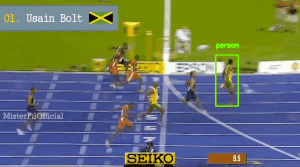
\includegraphics[width=0.5\textwidth]{img/chapters/estado-del-arte/sot-usain-bolt.png}
\caption{\label{fig:sot-usain-bolt}Ejemplo seguimiento de una única persona \cite{object-tracking-dlib}}
\end{figure}

\subsection{Seguimiento de múltiples objetos}
\label{subsec:seguimiento-multiples-objeto}

En \gls{mot}, como su nombre lo indica, se rastrean varios objetos al mismo tiempo. Se espera a que el algoritmo de seguimiento primero determine la cantidad de objetos en cada fotograma y, posteriormente, realice un seguimiento del ID de cada objeto de un fotograma al siguiente.

\gls{mot} es un problema desafiante ya que los cambios de ID son difíciles de evitar, especialmente en vídeos de grandes aglomeraciones de personas, donde se desconoce la naturaleza y la cantidad de objetos en cada fotograma. Los algoritmos \gls{mot} se basan en gran medida en algoritmos de detección, los cuales no son perfectos.

\begin{figure}[ht]
\centering
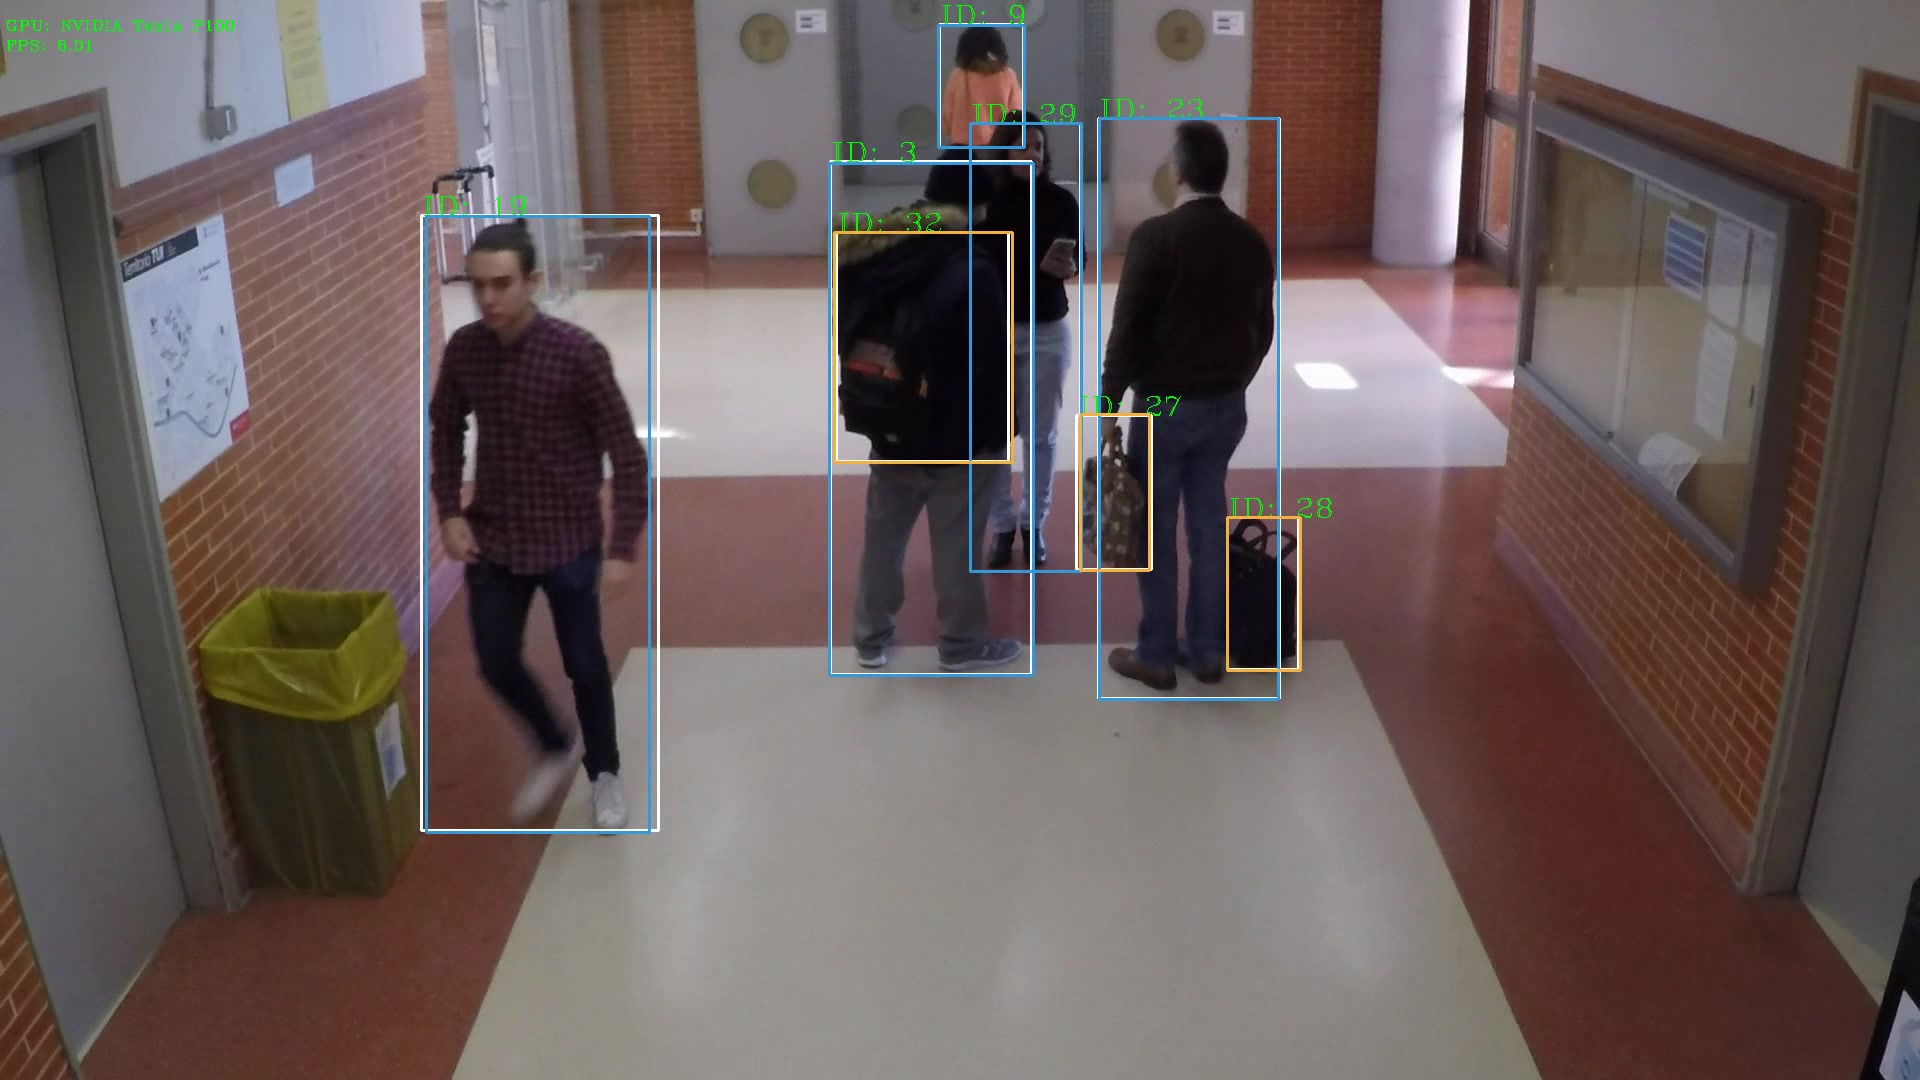
\includegraphics[width=0.5\textwidth]{img/chapters/estado-del-arte/mot-gba.jpg}
\caption{\label{fig:mot-gba}Ejemplo seguimiento de personas y objetos de interés en \cite{gba-dataset}}
\end{figure}

\subsection{Métodos tradicionales}
\label{subsec:metodos-tradicionales-seguimiento}

\subsubsection*{Mean Shift}
\label{subsubsec:mean-shift}

Mean Shift es un algoritmo iterativo no paramétrico y versátil que se puede usar para muchos propósitos, como modos de búsqueda o clusterings. Se ha utilizado ampliamente en el campo de seguimiento de objetivos debido a algunas ventajas como menos tiempos de iteración y mejor rendimiento en tiempo real. Sin embargo, debido a que solo se ha utilizado la representación de histograma de un solo color de la característica de destino en el algoritmo de Mean Shift, no se puede rastrear muy bien en algunos casos, especialmente en condiciones muy complicadas. Existen principalmente dos problemas que pueden hacer que el algoritmo de cambio medio tradicional sea inestable. El primer problema es cuando el color de fondo y el color de destino son similares, el rendimiento de seguimiento es significativamente insuficiente, el segundo es el problema de la oclusión parcial.

\subsubsection*{Optical Flow}
\label{subsubsec:optical-flow}

Optical Flow es el patrón de movimiento aparente de los objetos de la imagen entre dos fotogramas consecutivos causado por el movimiento del objeto o la cámara. El seguimiento con Optical Flow se basa en tres supuestos importantes:

\begin{itemize}
    \item Consistencia de brillo: se supone que el brillo alrededor de una región pequeña permanece casi constante, aunque la ubicación de la región puede cambiar.
    \item Coherencia espacial: los puntos vecinos en la escena normalmente pertenecen a la misma superficie y, por lo tanto, suelen tener movimientos similares.
    \item Persistencia temporal: el movimiento de un parche tiene un cambio gradual.
    \item Movimiento limitado: los puntos no se mueven muy lejos o de forma desordenada.
\end{itemize}

Una vez que se satisfacen estos criterios, se usa método de Lucas-Kanade para obtener una ecuación para la velocidad de los puntos que se van a rastrear y, junto a técnicas de predicción, se puede rastrear un objeto dado a lo largo del vídeo.

\subsection{Deep SORT}
\label{subsec:deepsort-algorithm}

\gls{deepsort} \cite{Wojke2017simple} es un algoritmo reciente para el seguimiento que amplía \gls{sort} \cite{Bewley_2016} y ha mostrado resultados notables en el problema de \gls{mot}.

\gls{sort} es un framework simple que emplea filtros de Kalman en el espacio de la imagen y la asociación de datos fotograma a fotograma utilizando el algoritmo húngaro con una métrica de asociación que mide el solapamiento del cuadro delimitador. Esta sencilla estrategia consigue un rendimiento favorable a altas velocidades de fotogramas. En el dataset del reto \gls{mot} \cite{lealtaixe2015motchallenge}, \gls{sort} junto con Faster \gls{r-cnn} se sitúa por encima de \gls{mht} en las detecciones estándar. Esto remarca la influencia del rendimiento del detector de objetos en los resultados generales del seguimiento.

Aunque consigue un buen rendimiento general en términos de precisión y exactitud del seguimiento, \gls{sort} devuelve un número relativamente alto de cambios de ID. Esto se debe a que la métrica de asociación empleada sólo es precisa cuando la incertidumbre en la estimación del estado es baja. Por lo tanto, \gls{sort} tiene una deficiencia en el seguimiento a través de oclusiones, tal y como suelen aparecer en escenas de cámaras de vista frontal. Este problema se soluciona sustituyendo la métrica de asociación por una métrica más informada que combina la información sobre el movimiento y la apariencia. Aplicando una \gls{cnn} se aumenta la robustez frente a fallos y oclusiones, manteniendo el sistema fácil de implementar, eficiente y aplicable a los escenarios en tiempo real.

\gls{deepsort} adopta una metodología convencional de seguimiento de una sola hipótesis con filtro de Kalman recursivo y asociación de datos fotograma a fotograma. En la siguientes secciones se describirá con más detalle los componentes principales de este sistema.

\subsubsection*{Tratamiento de los rastreos y estimación de estado}
\label{subsubsec:track-handling-and-state-estimation}

El marco de tratamiento de rastreos y el filtro de Kalman son mayormente idénticos a la formulación original de \gls{sort} \cite{Bewley_2016}. Se supone un escenario de seguimiento muy general en el que la cámara no está calibrada y no se dispone de información del \textit{egomotion}. Aunque estas circunstancias suponen un reto para el marco de filtrado, es la configuración más común considerada en los recientes benchmarks de \gls{mot} \cite{milan2016mot16}. El escenario de seguimiento se define en el espacio de estado de ocho dimensiones $(u,v,\gamma,h,\dot{u},\dot{v},\dot{\gamma},\dot{h})$ que contiene la posición del centro al cuadro delimitador $(u,v)$, la relación de aspecto $\gamma$, la altura $h$ y sus respectivas velocidades en coordenadas de imagen. Se utiliza un filtro de Kalman estándar con movimiento de velocidad constante y un modelo de observación lineal, en el que se toma las coordenadas de delimitación $(u,v,\gamma,h)$ como observaciones directas del estado del objeto.

Para cada rastreo $k$ se cuenta con un número de fotogramas desde la última asociación con éxito de la medición $a_{k}$. Este contador se incrementa durante la predicción del filtro de Kalman y se pone a cero cuando la pista se ha asociado a una medición. Se considera que los rastreos que superan una edad máxima predefinida $A_{\text{max}}$ han abandonado la escena y se eliminan del conjunto de rastreos. Se inician nuevas hipótesis de rastreos para cada detección que no puede asociarse a un rastreo existente. Estos nuevos rastreos se clasifican como tentativas durante sus tres primeros fotogramas. Durante este tiempo, se espera una asociación exitosa de la medición en cada paso de tiempo. Los rastreos que no se asocian con éxito a una medición dentro de los tres primeros fotogramas se eliminan.

\subsubsection*{Problema de asignación}
\label{subsubsec:assignment-problem}

Una forma convencional de resolver la asociación entre los estados de Kalman predichos y las mediciones llegadas es construir un problema de asignación que pueda resolverse mediante el algoritmo húngaro. En la formulación del problema se integra la información sobre el movimiento y la apariencia mediante la combinación de dos métricas adecuadas.

Para incorporar la información de movimiento se utiliza la distancia (al cuadrado) de Mahalanobis entre los estados de Kalman predichos y las nuevas mediciones llegadas:

\begin{equation}
\label{eq:equation1-deepsort}
d^{(1)} (i,j) = (\boldsymbol{d}_{j} - \boldsymbol{y}_{i})^{\text{T}} \boldsymbol{S}_{i}^{-1} (\boldsymbol{d}_{j} - \boldsymbol{y}_{i}),
\end{equation}

donde se denota la proyección de la $i$-th distribución del rastreo en el espacio de medición por $(\boldsymbol{y}_{i}, \boldsymbol{S}_{i})$ y la $j$-th detección del cuadro delimitador por $\boldsymbol{d}_{j}$. La distancia Mahalanobis tiene en cuenta la incertidumbre de la estimación del estado midiendo cuantas desviaciones estándar se aleja la detección de la ubicación media del rastreo. Además, utilizando esta métrica es posible excluir las asociaciones poco probables mediante el umbral de la distancia de Mahalanobis en un intervalo de confianza del 95\% calculado a partir de la inversa de distribución $\chi^{2}$. Se denota esta decisión con un indicador:

\begin{equation}
\label{eq:equation2-deepsort}
b_{i,j}^{(1)} = \mathbbm{1}[d^{(1)} (i,j) \leq t^{(1)}]
\end{equation}

que evalua a 1 si la asociación entre el rastreo $i$-th y la detección $j$-th es admisible. Para el espacio de medición cuatridimensional el umbral de Mahalanobis correspondiente es $t^{(1)} = 9,4877$.

Mientras que la distancia de Mahalanobis es una métrica de asociación adecuada cuando la incertidumbre del movimiento es baja, la formulación del problema del espacio de la imagen de distribución de estado predicha obtenida del marco de filtrado de Kalman sólo proporciona una estimación aproximada de la ubicación del objeto. En particular, el movimiento de la cámara de movimiento puede introducir desplazamientos rápidos en el plano de la imagen, lo que hace que la distancia de Mahalanobis sea una métrica poco informada para el seguimiento a través de oclusiones. Por tanto, se integra una segunda métrica en el problema de asignación. Para cada cuadro de detección $\boldsymbol{d}_{j}$ se calcula un descriptor de apariencia $\boldsymbol{r}_{j}$ con $\parallel \boldsymbol{r}_{j} \parallel = 1$. Además, se mantiene una galería $\mathcal{R}_{k} = \{\boldsymbol{r}_{k}^{(i)}\}_{k=1}^{L_{k}}$ de los últimos $L_{k} = 100$ descriptores de apariencia asociados a cada rastreo $k$. Por tanto, la segunda métrica mide la menor distancia del coseno entre el rastreo $i$-th y la detección $j$-th en el espacio de apariencia:

\begin{equation}
\label{eq:equation3-deepsort}
d_{i,j}^{(2)} = \text{min} \{1 - \boldsymbol{r}_{j}^{\text{T}} \boldsymbol{r}_{k}^{(i)} \ | \ \boldsymbol{r}_{k}^{(i)} \in \mathcal{R}_{i} \}.
\end{equation}

Se introduce una variable binaria para indicar si una asociación es admisible según esta métrica:

\begin{equation}
\label{eq:equation4-deepsort}
b_{i,j}^{(2)} = \mathbbm{1}[d^{(2)} (i,j) \leq t^{(2)}]
\end{equation}

y se encuentra un umbral adecuado para este indicador en un conjunto de datos de entrenamiento separado. En la práctica, se aplica una \gls{cnn} previamente capacitada para calcular los descriptores de apariencia del cuadro delimitador. La arquitectura de la red se explica en la sección \ref{subsubsec:deep-appearance-descriptor}.

En combinación, ambas métricas se complementan sirviendo diferentes aspectos del problema de asignación. Por un lado, la distancia de Mahalanobis proporciona información sobre las posibles ubicaciones de los objetos basadas en el movimiento que son especialmente útiles para las predicciones a corto plazo. Por otro lado, la distancia del coseno tiene en cuenta la información de la apariencia que son particularmente útiles para recuperar identidades después de oclusiones a largo plazo, cuando el movimiento es menos discriminatorio. Para construir el problema de asociación se combina ambas técnicas mediante una suma ponderada:

\begin{equation}
\label{eq:equation5-deepsort}
c_{i,j} = \lambda \ d^{(1)}(i,j) + (1 + \lambda)d^{(2)}(i,j)
\end{equation}

donde se considera asociación admisible si se encuentra dentro de la puerta regional de ambas métricas:

\begin{equation}
\label{eq:equation6-deepsort}
b_{i,j} = \prod_{m=1}^{2} b_{i,j}^{(m)}.
\end{equation}

La influencia de cada métrica en el coste de asociación combinado se puede controlar mediante el hiperparámetro $\lambda$. Se establece un $\lambda = 0$ cuando hay un movimiento sustancial de la cámara. Con esta configuración solo se usa información de apariencia en el término de coste de asociación. Sin embargo, la puerta de Mahalanobis todavía se usa para ignorar asignaciones no factibles basadas en posibles ubicaciones de objetos inferidas por el filtro de Kalman.

\subsubsection*{Matching Cascade}
\label{subsubsec:matching-cascade}

En lugar de resolver las asociaciones de medidas de rastreos en un problema de asignación global, se introduce una cascada que resuelve una serie de subproblemas. Se considera que cuando un objeto está ocluido durante un periodo de tiempo más largo, las predicciones posteriores del filtro Kalman aumentan la incertidumbre asociada a la localización del objeto. En consecuencia, la masa de probabilidad se extiende en el espacio de estados y la probabilidad de la observación se vuelve más baja. Intuitivamente, la métrica de asociación debería tener en cuenta esta dispersión de la masa de probabilidad aumentando la distancia de medición del rastreo. De forma contraria a la intuición, cuando dos rastreos compiten por la misma detección, la distancia de Mahalanobis favorece una mayor incertidumbre, porque reduce la distancia en desviaciones estándar de cualquier detección hacia la media del rastreo proyectado. Este es un comportamiento no deseado, ya que puede conducir a un aumento de las fragmentaciones de los rastreos y a la inestabilidad de las mismas. Por lo tanto, se introduce una cascada de coincidencia que da prioridad a los objetos vistos con más frecuencia para codificar la noción de dispersión de probabilidades en la probabilidad de asociación.

En la figura \ref{fig:matching-cascade} se recalca el algoritmo de emparejamiento. Como entrada se proporciona el conjunto de índices de rastreos $\mathcal{T}$ y detecciones $\mathcal{D}$ así como la edad máxima $A_{\text{max}}$. En las líneas 1 y 2 se calcula la matriz de costes de asociación y la matriz de asociaciones admisibles. A continuación, se itera sobre la edad del rastreo $n$ para resolver un problema de asignación lineal para rastreos de edad creciente. En la línea 6 se selecciona el subconjunto de rastreos $\mathcal{T}_{n}$ que no han sido asociadas a una detección en los últimos $n$ fotogramas. En la línea 7 se resuelve la asignación lineal entre $\mathcal{T}_{n}$ y las detecciones no coincidentes $\mathcal{U}$.

En las líneas 8 y 9 se actualiza el conjunto de coincidencias y detecciones no coincidentes, que se devuelve tras la finalización en la línea 11.

En la etapa final de emparejamiento, se ejecuta la \gls{iou} en el conjunto de rastreos no confirmados y no emparejados de edad $n = 1$. Esto ayuda a tener en cuenta los cambios repentinos de apariencia, por ejemplo, debido a la oclusión parcial con la geometría estática de la escena, y a aumentar la robustez contra la inicialización errónea.

\begin{figure}[ht]
\centering
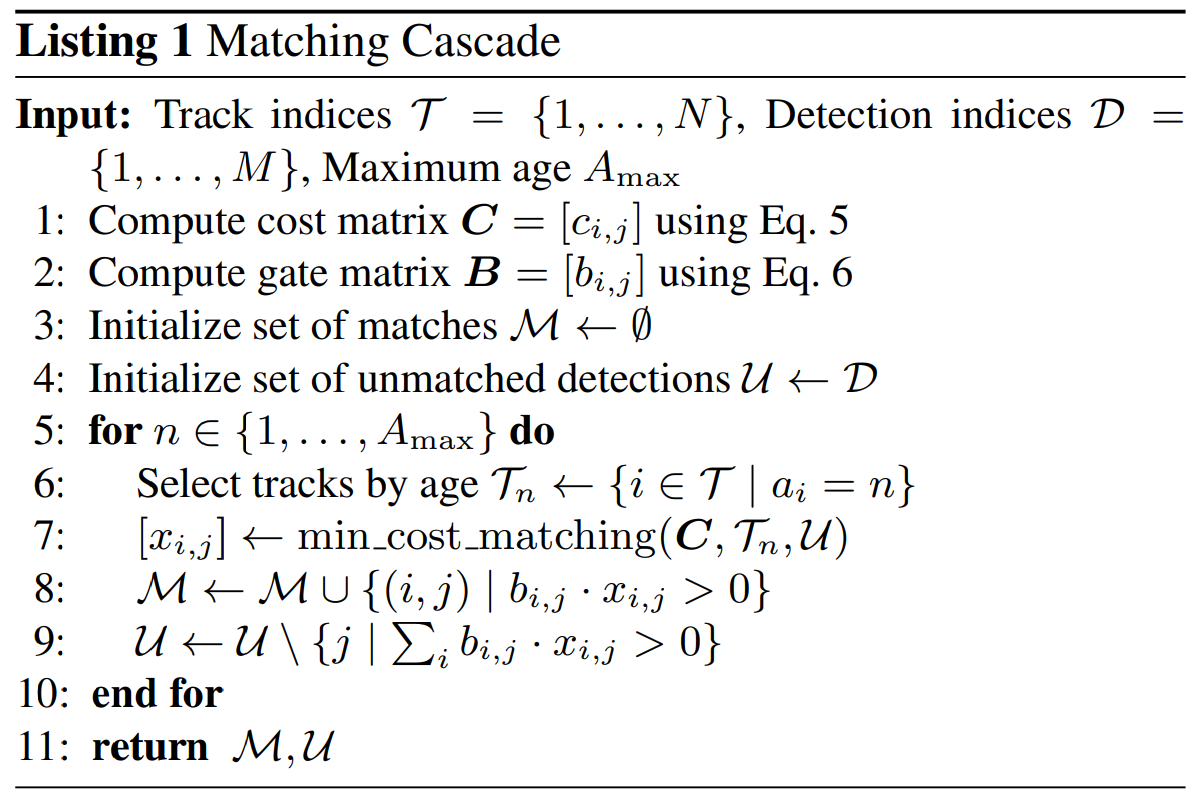
\includegraphics[width=0.6\textwidth]{img/chapters/estado-del-arte/matching-cascade.png}
\caption{\label{fig:matching-cascade}Matching Cascade \cite{Wojke2017simple}}
\end{figure}

\subsubsection*{Descriptor de apariencia profunda}
\label{subsubsec:deep-appearance-descriptor}

Mediante el uso de consultas simples al vecino más cercano sin aprendizaje métrico adicional, se requiere una incrustación de características discriminante que debe ser entrenada fuera de línea, antes de la aplicación real de seguimiento en línea. En la versión original de \gls{deepsort}, se empleó una \gls{cnn} entrenada en el dataset de reidentificación de personas MARS \cite{10.1007/978-3-319-46466-4_52} que contiene más de 1.100.000 imágenes de 1.261 peatones, lo que la hace muy adecuada para el aprendizaje métrico profundo en un contexto de seguimiento de personas.

\begin{table}[ht]
\centering
\caption{Batch final con normalización $\ell_2$ proyectan las características en la hiperesfera unitaria \cite{Wojke2017simple}}
\label{tab:final-bach-l2-normalization}
\begin{tabular}{lcc}
\hline
\textbf{Name}                    & \textbf{Patch Size/Stride} & \textbf{Output Size} \\ \hline
Conv 1                           & 3 x 3/1                    & 32 x 128 x 64        \\
Conv 2                           & 3 x 3/1                    & 32 x 128 x 64        \\
Max Pool 3                       & 3 x 3/2                    & 32 x 64 x 32         \\
Residual 4                       & 3 x 3/1                    & 32 x 64 x 32         \\
Residual 5                       & 3 x 3/1                    & 32 x 64 x 32         \\
Residual 6                       & 3 x 3/2                    & 64 x 32 x 16         \\
Residual 7                       & 3 x 3/1                    & 64 x 32 x 16         \\
Residual 8                       & 3 x 3/2                    & 128 x 16 x 8         \\
Residual 9                       & 3 x 3/1                    & 128 x 16 x 8         \\
Dense 10                         &                            & 128                  \\
Batch and $\ell_2$ normalization &                            & 128                  \\ \hline
\end{tabular}
\end{table}

La arquitectura de la \gls{cnn} de la red se muestra en la tabla \ref{tab:final-bach-l2-normalization}. Se trata de una red residual amplia con dos capas convolucionales seguidas de seis bloques residuales. El mapa global de características de dimensionalidad 128 se computa en la capa densa 10. Un batch final y una normalización $\ell_2$ proyectan los rasgos en la hiperesfera unitaria para que sean compatibles con la métrica de apariencia del coseno. En total la red tiene 2.800.864 parámetros, y el pase de avance de 32 cuadros delimitadores tarda aproximadamente 30 ms en una \gls{gpu} NVIDIA GeForce GTX 1050. Esta red es muy adecuada para el seguimiento en línea, siempre que se disponga de una \gls{gpu} moderna.
